\chapter{Geometría Diferencial de las Superficies}

\section{Aspectos locales}

\begin{defn}
Una \textbf{carta} es una función $\x:U\subseteq\RR^2\to\RR^3$ definida en un abierto $U\subseteq \RR^2$ que es inyectiva, diferenciable y tal que para todo $u\in U$ tenemos que $\partial_1 \x(u)\wedge \partial_2 \x(u) \neq 0$, donde $\partial_1 \x,\partial_2 \x$ son las derivadas parciales de $\x$ respecto de la primera y segunda coordenada respectivamente. Esto es equivalente a que los vectores $\{\partial_1 \x(u),\partial_2 \x(u)\}$ sean linealmente independientes. La imagen de $\x$ se denomina la \textbf{traza} de la carta.
\end{defn}

\begin{defn}
Sea $\x:U\subseteq\RR^2\to\RR^3$ una carta. Las funciones $\x_1=\partial_1 \x:U\to\RR^3$ y $\x_2=\partial_2\x:U\to\RR^3$ se denominan \textbf{campos coordenados} y la función $\n:U\to\RR^3$ dada por $\n(u)=\dfrac{\x_1(u)\wedge \x_2(u)}{\norm{\x_1(u)\wedge \x_2(u)}}$ es el denominado \textbf{campo normal unitario}.
\end{defn}

\begin{defn}
Un \textbf{cambio de coordenadas} es una función $\varphi:V\to U$ entre abiertos del plano $U,V\subseteq\RR^2$ que es biyectiva, diferenciable y con inversa diferenciable.
\end{defn}

Supongamos que $\varphi:V\to U$ es un cambio de coordenadas. La función $\varphi$ está determinada por sus componentes $\varphi^1,\varphi^2:V\to\RR$. Es decir, $\varphi(v)=(\varphi^1(v),\varphi^2(v))$ para cada $v\in V$. Recordemos que se define la \textbf{diferencial} de una función $\varphi$ como la asignación $\D_\varphi:V\to\mathscr{M}_2(\RR)$ dada por: $$\D_\varphi(v)=\begin{pmatrix}\partial_1 \varphi^1(v) & \partial_2 \varphi^1(v)\\ \partial_1 \varphi^2(v) & \partial_2 \varphi^2(v)\end{pmatrix}$$
Recordemos también que el determinante de la matrix $\J_\varphi(v)=\det\D_\varphi(v)$ se denomina el \textbf{jacobiano} de $\varphi$. Si $\psi:U\to V$ es la inversa diferenciable de $\varphi:V\to U$, entonces $\psi\circ\varphi(v)=v$ para cada $v\in V$ y por la regla de la cadena tenemos que $\D_\psi(\varphi(v)) \D_\varphi(v)=I$ donde $I\in\mathscr{M}_2(\RR)$ es la matriz identidad. Más concretamente, se tiene que $\displaystyle\sum_{k=1}^2 \dfrac{\partial \psi^i}{\partial u^k}(\varphi(v)) \dfrac{\partial\varphi^k}{\partial v^j}(v) = \delta_{j}^{i}$ para cada $i,j\in\{1,2\}$ (donde $\delta_i^j$ es la delta de Kronecker).
En particular, tenemos que $\D_\varphi(v)\in\GL_2(\RR)$ y así $\J_\varphi(v)$ nunca se anula. Por lo tanto, la asignación $\J_\varphi:V\to\RR$ es continua (pues tomar determinante es una función en términos de las coordenadas de la matriz y así es claramente continuo y $\D_\varphi$ es continua asumiendo regularidad al menos $\mathscr{C}^1$ de $\varphi$). Si $V$ es conexo y como $\J_\varphi$ nunca se anula, debe ser que $\J_\varphi$ tiene signo constante. En el caso que $\J_\varphi>0$ se dice que $\varphi$ \textbf{preserva la orientación}, mientras que si $\J_\varphi<0$ decimos que $\varphi$ \textbf{invierte la orientación}.

\begin{prop}\label{prop::cartacambiodecoordenadas}
Si $\x:U\to\RR^3$ es una carta y $\varphi:V\to U$ es un cambio de coordenadas, entonces $\y=\x\circ\varphi:V\to\RR^3$ también es una carta y tiene la misma traza que $\x$. Más aún, tenemos que $\y_i = \displaystyle\sum_{j=1}^2 \partial_i \varphi^j \x_j$, y el campo normal a $\y$ es $\n$ o $-\n$ dependiendo de si $\varphi$ preserva o revierte la orientación respectivamente.
\begin{proof}
Claramente $\y$ es diferenciable por ser composición de funciones diferenciables, e inyeciva por la razón análoga. Ahora, por la regla de la cadena tenemos que: $$\y_i(v)=\partial_i\y(v)=\partial_i (\x\circ\varphi)(v)=\displaystyle\sum_{j=1}^2 \dfrac{\partial\x}{\partial u^j}(\varphi(v))\dfrac{\partial\varphi^j}{\partial v^i}(v) = \displaystyle\sum_{j=1}^2 \partial_i\varphi^j(v)\x_j(\varphi(v))$$ Entonces, para ver que es una carta, sólamente falta ver que $\y_1\wedge\y_2\neq 0$. Calculemos este producto vectorial:
\begin{align*}
\y_1\wedge\y_2 &= \left(\displaystyle\sum_{j=1}^2 \partial_1 \varphi^j\x_j\right)\wedge\left(\displaystyle\sum_{k=1}^2 \partial_2 \varphi^k\x_k\right) \\ &= \left(\partial_1\varphi^1\x_1\wedge\partial_2\varphi^2\x_2\right) + \left(\partial_1\varphi^2\x_2\wedge\partial_2\varphi^1\x_1\right)\\
&=\left(\partial_1\varphi^1\partial_2\varphi^2 - \partial_1\varphi^2\partial_2\varphi^1\right) \x_1\wedge \x_2\\
&= \J_\varphi \x_1\wedge\x_2
\end{align*}
Esto es no nulo por ser $\J_\varphi(v)\neq 0$ para todo $v\in V$ y $\x_1(v)\wedge\x_2(v)\neq 0$ por ser $\x$ una carta. Finalmente, el campo normal de $\y$ es simplemente $\dfrac{\y_1\wedge\y_2}{\norm{\y_1\wedge\y_2}} = \dfrac{\J_\varphi}{|\J_\varphi|}\dfrac{\x_1\wedge\x_2}{\norm{\x_1\wedge\x_2}} = \sg(\J_\varphi)\n$. Esto concluye la demostración.
\end{proof}
\end{prop}

\begin{defn}
Si $\x:U\to\RR^3$ es una carta y $X\in\RR^3$ un vector, decimos que $X$ es \textbf{tangente} a $\x$ en $u\in U$ si existe $\varepsilon>0$ y $\alpha:(-\varepsilon,\varepsilon)\to U$ diferenciable tal que $\alpha(0)=u$ y $X = (\x\circ\alpha)'(0)$.
\begin{figure}[h]
	\centering
		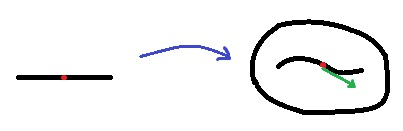
\includegraphics[width=0.48\textwidth]{C:/Users/Nacho/Documents/Latex/Facultad/GeometriaProyectiva/GeoProyectiva/vectortangentesuperficie.jpg}
	\caption{Un vector tangente a una carta $\x$ visto como la velocidad de una curva.}
	\label{fig:vectortangentesuperficie}
\end{figure}
\end{defn}

\begin{prop}
Sea $\x:U\to\RR^3$ una carta y $u\in U$. El conjunto $\mathrm{T}_{u}\x$ de todos los vectores tangentes a $\x$ en $u\in U$ es un subespacio vectorial de $\RR^3$ de dimensión $2$ que tiene al conjunto $\{\x_1(u),\x_2(u)\}$ como base y que es ortogonal a $\n(u)$.
\begin{proof}
Notemos primero que $\x_1(u),\x_2(u)\in\mathrm{T}_u\x$. En efecto, considero $\xi_1:\RR\to\RR^2$ dada por $\xi_1(t)=(u^1+t,u^2)$. Como $\xi_1(0)=(u^1,u^2)=u$ y $U$ es abierto, existe un $\varepsilon>0$ tal que $\xi_1$ se restringe a $\xi_1:(-\varepsilon,\varepsilon)\to U$. Es fácil comprobar que $(\x\circ\xi_1)'(0)=\x_1(u)$. De manera análoga, considerando $\xi_2(t)=(u^1,u^2+t)$ y restringiéndola a un entorno adecuado se sigue que $(\x\circ\xi_2)'(0)=\x_2(u)$. Esto implica que $\x_1(u),\x_2(u)\in\mathrm{T}_u\x$.

Sean $X,Y\in\mathrm{T}_u\x$ y $\lambda\in\RR$. Por lo tanto, existen $\alpha,\beta:(-\varepsilon,\varepsilon)\to U\subseteq\RR^2$ funciones tales que $\alpha(0)=\beta(0)=u$ y $X=(\x\circ\alpha)'(0)$, $Y=(\x\circ\beta)'(0)$. Por la regla de la cadena, podemos escribir esto de forma más concisa como $X=(\alpha^1)'(0)\x_1(u) + (\alpha^2)'(0)\x_2(u)$ e $Y=(\beta^1)'(0)\x_1(u)+(\beta^2)'(0)\x_2(u)$. Veamos que $X+\lambda Y\in\mathrm{T}_u\x$. Para ello, consideremos $\gamma:\RR\to\RR^2$ dada por $\gamma(t)=\alpha(t)+\beta(\lambda t)-u$. Como $\gamma(0)=u\in U$ y $U$ es abierto, podemos considerar la restricción $\gamma:(-\varepsilon',\varepsilon')\to U$ para algún $\varepsilon'>0$. Ahora bien, por la regla de la cadena sabemos que: \begin{align*}(\x\circ\gamma)'(0)&=(\gamma^1)'(0)\x_1(u)+(\gamma^2)'(0)\x_2(u)\\ &= \left((\alpha^1)'(0)+\lambda (\beta^1)'(0)\right)\x_1(u) + \left((\alpha^2)'(0)+\lambda (\beta^2)'(0)\right)\x_2(u) = X+\lambda Y\end{align*} 
Y así $\mathrm{T}_u\x$ forma un espacio vectorial. Por otra parte, a cualquier elemento de $\mathrm{T}_u\x$ lo pudimos expresar como combinación lineal de $\{\x_1(u),\x_2(u)\}$, que son linealmente independientes por la definición de carta. Esto concluye la demostración.
\end{proof}
\end{prop}

\begin{defn}
Si $\x:U\to\RR^3$ es una carta, decimos que el espacio vectorial $\mathrm{T}_u\x$ de dimensión $2$ es el \textbf{plano tangente} a $\x$ en $u$.
\end{defn}

\begin{prop}
Sea $\x:U\to\RR^3$ una carta y sea $\varphi:V\to U$ un cambio de coordenadas y sea $\y=\x\circ\varphi: V\to \RR^3$. Si $v\in V$, entonces los espacios $\mathrm{T}_v\y = \mathrm{T}_{\varphi(v)}\x$ coinciden. Más aún, si $X\in\mathrm{T}_v\y$ y escribimos $X = X^1\x_1(\varphi(v)) + X^2\x_2(\varphi(v)) = Y^1\y_1(\varphi(v)) + Y^2\y_2(\varphi(v))$. Entonces, $X^i = \displaystyle\sum_{j=1}^2 \partial_j\varphi^i Y^j$, o dicho de otra forma: $$\begin{pmatrix}X^1 \\ X^2\end{pmatrix} = \D_\varphi(v)\begin{pmatrix}Y^1 \\ Y^2\end{pmatrix}$$
\begin{proof}
Sea $X\in\mathrm{T}_v\y$. Luego, existen $\varepsilon>0$ y $\alpha:(-\varepsilon,\varepsilon)\to V$ tales que $\alpha(0)=v$ y $X=(\y\circ\alpha)'(0)$. Pero como $\y=\x\circ\varphi$, se tiene que $(\x\circ (\varphi\circ\alpha))'(0)$ y $\varphi\circ\alpha:(-\varepsilon,\varepsilon)\to U$ es una curva con $\varphi\circ\alpha(0)=\varphi(v)$, tenemos que $X\in\mathrm{T}_{\varphi(v)}\x$. Por lo tanto, $\mathrm{T}_v\y\subseteq\mathrm{T}_{\varphi(v)}\x$. Como son espacios vectoriales de dimensión $2$, deben ser iguales.

Ahora bien, para ver la otra parte de la proposición, utilizamos el cambio de coordenadas que nos da la Proposición ~\ref{prop::cartacambiodecoordenadas}: $$\displaystyle\sum_{i=1}^2 X^i \x_i(\varphi(v)) = \displaystyle\sum_{j=1}^2 Y^j \y_j(v)=\displaystyle\sum_{j=1}^2 Y^j \left(\displaystyle\sum_{i=1}^2 \partial_j\varphi^i \x_i(\varphi(v))\right) = \displaystyle\sum_{i=1}^2 \left(\displaystyle\sum_{j=1}^2 \partial_j\varphi^i Y^j\right)\x_i(\varphi(v))$$

Como queríamos probar.
\end{proof}
\end{prop}

\begin{prop}\label{prop::tangenteconcartas}
Sea $\x:U\to\RR^3$ una carta y $u\in U$ y fijemos $X\in\mathrm{T}_u\x$. Entonces:
\begin{enumerate}
\item Sea $f\in\mathscr{C}^\infty(U,\RR^n)$. Si $\varepsilon>0$ y $\alpha:(-\varepsilon,\varepsilon)\to U$ son tales que $\alpha(0)=u$ y $(\x\circ\alpha)'(0)=X$, entonces el elemento $(f\circ\alpha)'(0)\in\RR^n$ sólo depende de $X$ y de $f$ y \textbf{no} de la elección de $\alpha$ y $\varepsilon$. Denotamos luego $Xf=(f\circ\alpha)'(0)$.
\item Si $X^1,X^2\in\RR$ son tales que $X=\displaystyle\sum_{i=1}^2 X^i\x_i(u)$, entonces $Xf = \displaystyle\sum_{i=1}^2 X^i\partial_i f(u)$.
\item La función $\mathscr{C}^\infty(U,\RR^n)\to\RR^n$ dada por $f\mapsto Xf$ es $\RR$-lineal.
\item Si $f\in\mathscr{C}^\infty(U,\RR)$ y $g\in\mathscr{C}^\infty(U,\RR^n)$, entonces $X(fg)=Xf\, g(u) + f(u)Xg$.
\end{enumerate}
\begin{proof}
\hfill

\begin{enumerate}
\item Sean $\varepsilon>0$, $\alpha,\beta:(-\varepsilon,\varepsilon)\to U$ tales que se cumple que $\alpha(0)=\beta(0)=u$ y $(\x\circ\alpha)'(0)=X=(\x\circ\beta)'(0)$. Más concretamente, esto se puede escribir como $\displaystyle\sum_{i=1}^2 (\alpha^i)'(0)\x_i(u) = \displaystyle\sum_{i=1}^2 (\beta^i)'(0)\x_i(u)$. Usando que $\{\x_1(u),\x_2(u)\}$ es una base, tenemos que $(\alpha^i)'(0)=(\beta^i)'(0)$.
Sea $f\in\mathscr{C}(U,\RR^n)$. Veamos que $(f\circ\alpha)'(0)=(f\circ\beta)'(0)$, esto implicará la buena definición $Xf$. Pero esto es: $$(f\circ\alpha)'(0)=\displaystyle\sum_{i=1}^2 (\alpha^i)'(0)\partial_i f(u) = \displaystyle\sum_{i=1}^2 (\beta^i)'(0)\partial_{i} f(u)=(f\circ\beta)'(0)$$
\item Sea $\gamma:\RR\to\RR^2$ dada por $\gamma(t)=u+t(X^1,X^2)$. Como $\gamma(0)=u\in U$ y $U$ es abierto, podemos restringirnos a $\gamma:(-\varepsilon,\varepsilon)\to U$. Además, tenemos que: $$(\x\circ\gamma)'(0)=\displaystyle\sum_{i=1}^2 (\gamma^i)'(0)\x_i(u) = \displaystyle\sum_{i=1}^2 X^i \x_i(u)=X$$ Por lo tanto, por el item 1, $Xf=(f\circ\gamma)'(0)$ y es fácil corroborar, por la regla de la cadena, que $(f\circ\gamma)'(0)=\displaystyle\sum_{i=1}^2 (\gamma^i)'(0)\partial_i f(u)=\displaystyle\sum_{i=1}^2 X^i\partial_i f(u)$.
\item Por el item 2. tenemos que: \begin{align*}X(f+\lambda g)&=\displaystyle\sum_{i=1}^2 X^i \partial_i(f+\lambda g)(u)\\ &= \displaystyle\sum_{i=1}^2 X^i (\partial_i f(u)+ \lambda \partial_i g(u)) = \displaystyle\sum_{i=1}^2 X^i\partial_i f(u) + \lambda \displaystyle\sum_{i=1}^2 X^i\partial_i g(u) = Xf + \lambda Xg\end{align*}
\item Es inmediato con el item 2.\end{enumerate}\end{proof}
\end{prop}

\begin{defn}
Un conjunto $S\subseteq\RR^3$ es una \textbf{superficie} si para todo $p\in S$ existe una carta $\x:U\to\RR^3$ tal que:
\begin{itemize}
\item $p\in\x(U)\subseteq S$.
\item $\x(U)$ es un abierto de $S$.
\item La correstricción $\x:U\to\x(U)$ tiene inversa continua.
\end{itemize}
Una tal carta $\x$ se denomina una carta de $S$.
\end{defn}

\begin{prop}
Sea $S\subseteq\RR^3$ una superficie y $V\subseteq S$ un abierto de $S$. Entonces $V$ es una superficie.
\begin{proof}
Sea $p\in V$. Como $S$ es una superficie, existe $U\subseteq\RR^2$ abierto y $\x:U\to\RR^3$ una carta de $S$ tal que $p\in\x(U)$. Como $V$ es abierto en $S$ y $\x:U\to S$ es continua, entonces $\x^{-1}(V)$ es abierto. Consideremos $\y=\left.\x\right|_{\x^{-1}(V)}:\x^{-1}(V)\to\RR^3$. Claramente $\y$ es una carta, pues $\x^{-1}(V)$ es abierto, $\x$ es inyectiva y así su restricción lo es y $\partial_i\y(u)=\partial_i\x(u)$ para cada $u\in\x^{-1}(V)$, lo que implica que $\{\partial_1\y(u),\partial_2\y(u)\}$ son linealmente independientes por ser $\x$ una carta. 

Notemos que $p\in\y(\x^{-1}(V))$ pues $p\in V\cap\x(U)$. Además, $\y(\x^{-1}(V)) = V\cap\x(U)$, que es un abierto de $V$, por ser $\x(U)$ un abierto de $S$. Finalmente, $\y$ tiene inversa continua, pues simplemente es retringir la inversa de $\x$ a $V\cap\x^{-1}(V)$. Esto concluye la demostración.
\end{proof}
\end{prop}

\begin{prop}\label{prop::valoresregulares}
Sea $W\subseteq\RR^3$ abierto y $f:W\to\RR$ de clase $\mathscr{C}^\infty$. Entonces el conjunto $S=\{p\in\RR^3 : f(p)=0\}$ es una superficie para todo $p\in S$ tal que $\nabla f(p)\neq 0$.
\begin{proof}
El principal ingrediente de la demostración será el Teorema de la Función Inversa. Sea $p\in S$. Por hipótesis, $\nabla f(p)\neq 0$. Sin pérdida de la generalidad, supongamos que $\partial_3 f(p)\neq 0$. Sea $F:W\to\RR^3$ la función dada por $F(q^1,q^2) = (q^1,q^2,f(q^1,q^2))$. La diferencial de $F$ en $p$ está dada por la matriz $$\D F(p)=\begin{pmatrix}1&0&0\\0&1&0\\ \partial_1f(p)&\partial_2f(p)&\partial_3f(p)\end{pmatrix}$$ Esta matriz resulta inversible por ser $\partial_3f(p)\neq 0$. Por el Teorema de la Función Inversa, existen abiertos $A\subseteq W$, $B\subseteq\RR^3$ tales que $p\in A$, $F(A)=B$ y $F:A\to B$ es biyectiva, de clase $\mathscr{C}^\infty$ y con inversa de clase $\mathscr{C}^\infty$. Además, $\D F^{-1}(F(p))$ tiene por inversa a $\D F(p)$.

Consideremos el abierto $U=\{(u^1,u^2)\in\RR^2 : (u^1,u^2,0)\in B\}$, y sea $\x:U\to\RR^3$ dada por $\x(u^1,u^2)=F^{-1}(u^1,u^2,0)$. Esta función es de clase $\mathscr{C}^\infty$ por ser composición de funciones $\mathscr{C}^\infty$ y toma valores en $A$. Si $u,v\in V$ son tales que $\x(u)=\x(v)$, entonces $F^{-1}(u,0)=F^{-1}(v,0)$ y así $u=v$ por ser $F^{-1}$ inyectiva. Esto implica que $\x$ es inyectiva. Además, notemos que $\partial_i\x(q) = \D F^{-1}(q,0)e_i$ para cada $q\in U$. por lo tanto, $\partial_1\x(q)$ y $\partial_2\x(q)$ deben ser linealmente independientes por ser esa matriz inversible. Esto implica que $\x$ es una carta.

Ahora bien, si $u\in U$, por definición tenemos que $F(\x(u)) = (\x(u),f(\x(u)))$. Pero por otra parte, $F(\x(u)) = F(F^{-1}(u^1,u^2,0)) = (u^1,u^2,0)$. Por lo tanto, $f(\x(u))=0$ para cada $u\in U$. Es decir, $\x(U)\subseteq S$. Como $\x$ toma valores en $A$, tenemos que $\x(U)\subseteq A\cap S$. Recíprocamente, si $p\in A\cap S$, entonces $f(p)=0$ y así $F(p)=(p^1,p^2,0)$. Luego, esto implica que $\x(p)=F^{-1}(p^1,p^2,0)=F^{-1}(F(p))=p$. Es decir, $\x(U)=A\cap S$, y en particular es un abierto de $S$. Por último, consideremos la proyección $\pi:\RR^3\to\RR^2$, $\pi(x)=(x^1,x^2)$. Claramente es continua y $\pi(F(A\cap S))=U$. Si miro la restricción $\left.\pi\circ F\right|_{A\cap S}:A\cap S = \x(U)\to U$, entonces es fácil ver que $\pi\circ F$ es la inversa de $\x$. La proposición sigue.
\end{proof}
\end{prop}

\begin{ex}
La Proposición ~\ref{prop::valoresregulares} nos permite probar que la mayoría de las superficies que conocemos son de hecho superficies bajo nuestra definición. Por ejemplo, una esfera, $S=\{(x,y,z)\in\RR^3 : x^2+y^2+z^2 =1\}$ simplemente la podemos pensar como $f^{-1}(0)$ donde $f(x,y,z)=x^2+y^2+z^2-1$ pues $\nabla f(p)=(2p^1,2p^2,2p^3)$ sólo se anula si $p=0\notin S$. De manera similar podemos probar que un paraboloide $S=\{(x,y,z)\in\RR^3 : z = x^2+y^2\}$ es una superficie. En ambos casos, no tuvimos que exhibir un conjunto de cartas, y por eso la utilidad de esta Proposición. \textcolor{red}{Agregar cuentitas con cartas antes de la proposición}
\end{ex}

\begin{cor}
Sea $U\subseteq\RR^2$ un abierto y $f:U\to\RR$ una función diferenciable. El gráfico de $f$, $S=\{(u,f(u)) : u\in U\}\subseteq\RR^3$ es una superficie.
\begin{proof}
Sea $W=U\times\RR\subseteq\RR^3$ abierto y sea $F:U\times\RR\to\RR$, $F(u,t)=f(u)-t$. Es claro que $F^{-1}(0)=S$. Por otra parte, $\nabla F(u,t)=(\partial_1f(u),\partial_2f(u),-1)\neq 0$. Aplicando la Proposición ~\ref{prop::valoresregulares} ya estamos.
\end{proof}
\end{cor}

\begin{cor}
Toda superficie es localmente el gráfico de una función.
\begin{proof}
\textcolor{red}{HACER!}
\end{proof}
\end{cor}

El siguiente resultado técnico nos será muy útil. En esencia, nos permitirá extender funciones continuas sobre una superficie $S\subseteq\RR^3$ a funciones diferenciables en un entorno de un punto $p\in S\subseteq\RR^3$. \textcolor{red}{Escribir esto mejor...}

\begin{prop}\label{prop::ensanchetecnico}
Sea $S\subseteq\RR^3$ una superficie. Si $\x:U\to\RR^3$ es una carta tal que $\x(U)\subseteq S$, entonces $\x$ es una carta de $S$. Más aún, para cada $u\in U$ existe un abierto $W\subseteq\RR^3$ y una función diferenciable $r:W\to\RR^2$ tal que $\x(u)\in W\cap S\subseteq\x(U)$ y $\x^{-1}(q)=r(q)$ para todo $q\in W\cap S$.
\begin{proof}
Sea $u_0\in U$ y $p=\x(u_0)$. Como $S$ es una superficie, hay una carta de $S$, $\y:V\to S$ tal que $\y(v_0)=p$ para algún $v_0\in V$. También, existe $\Omega\subseteq\RR^3$ abierto tal que $\y(V)=\Omega\cap S$. Sea $\n:V\to\RR^3$ el campo normal a $\y$, y consideremos la función $\widetilde{\y}:V\times\RR\to\RR^2$ dada por $\widetilde{\y}(v,t)=\y(v)+t\n(v)$. Claramente se tiene que $\widetilde{\y}(v_0,0)=p$. También es fácil ver que $\partial_1\widetilde{\y}(v_0,0)=\partial_1\y(v_0)$, $\partial_2\widetilde{\y}(v_0,0) = \partial_2\y(v_0)$ y $\partial_3\widetilde{\y}(v_0,0)=\n(v_0)$. Estos tres vectores resultan ser linealmente independientes por ser $\y$ una carta. Por lo tanto, la matriz $\D\widetilde{\y}(v_0,0)$ es inversible.

\begin{figure}[h]
	\centering
		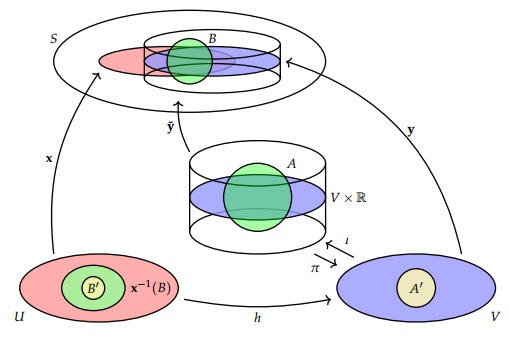
\includegraphics[width=0.60\textwidth]{C:/Users/Nacho/Documents/Latex/Facultad/GeometriaProyectiva/GeoProyectiva/dibuensanchetecnico.jpg}
	\caption{Un dibujo que ilustra la demostración de la Proposición ~\ref{prop::ensanchetecnico}}
	\label{fig:dibuensanchetecnico}
\end{figure}

Por lo tanto, existen abiertos $A\subseteq V\times\RR$, $B\subseteq\RR^3$ tales que $(v_0,0)\in A$, $\widetilde{\y}(v_0,0)\in B$ y además $\widetilde{\y}:A\to B$ es biyectiva, de clase $\mathscr{C}^\infty$ y su inversa también. Más aún, podemos suponer (por la demostración del Teorema de la Función Inversa) que $B\subseteq\Omega$. Es fácil ver que $\widetilde{\y}(V\times\{0\}) \subseteq S$ y $\widetilde{\y}^{-1}(B\cap S) \subseteq V\times\{0\}$. Como $\x$ es continua y $\x(u_0)\in B$, se tiene que $\x^{-1}(B)\subseteq U$ es un abierto de $U$ y $u_0\in\x^{-1}(B)$. Consideremos entonces $h:\x^{-1}(B)\to V$ dada por $h=\pi\circ\widetilde{\y}^{-1}\circ\x$, donde $\pi:V\times\RR\to V$ es la proyección en la primera coordenada. Sea $\iota:V\to V\times\{0\}$ la inclusión canónica. Notemos que $\iota\circ h = \widetilde{\y}^{-1}\circ\x$ sobre $\x^{-1}(B)$ por ser $\widetilde{\y}^{-1}(B\cap S) = V\times\{0\}$. Ahora bien, por regla de la cadena tenemos que $\D(\iota\circ h)(u_0)=\D\iota(h(u_0))\D h(u_0)$. Por otra parte, tenemos que $\D(\widetilde{\y}^{-1}\circ\x(u_0))=\D\widetilde{\y}^{-1}(\x(u_0))\D\x(u_0) = \D\widetilde{\y}^{-1}(p)\D\x(u_0)$. Como $\D\widetilde{\y}^{-1}(p)$ y $\D\x(u_0)$  son inyectivas, su producto (ie. composición) lo es y así $\D(\iota\circ h)(u_0)$ debe serlo. Esto implica que $\D h(u_0)$ es inyectivo. Pero como $h:\RR^2\to\RR^2$, $\D h(u_0)$ es una transformación lineal inyectiva entre espacios vectoriales de la misma dimensión. Es decir, $\D h(u_0)$ debe ser inversible. Aplicamos el Teorema de la Función Inversa nuevamente. Existen abiertos $B'\subseteq\x^{-1}(B)$, $A'\subseteq V$ con $u_0\in B'$, $h(B')=A'$ y $h:B'\to A'$ biyectiva de clase $\mathscr{C}^\infty$ con inversa de clase $\mathscr{C}^\infty$.

Como $\y\circ\pi\circ\widetilde{\y}^{-1}$ es la identidad, tenemos que: $$\x(B')=(\y\circ\pi\circ\widetilde{\y}^{-1}\circ\x)(B')=\y(h(B'))=\y(A')$$ Por lo tanto, $\x(B')$ es un abierto de $S$ por serlo $\y(A')$ ya que $\y$ es una carta de $S$. Notemos además que $p\in\x(B')$ pues $p\in\y(A')$. Como $p\in\x(B')\subseteq\x(U)$, tenemos que todo punto de $\x(U)$ es un punto interior por ser $\x(B')$ abierto en $S$. Es decir, $\x(U)$ es abierto en $S$.

Sólo resta ver que existen $W\subseteq\RR^3$ abierto tal que $\x(u)\in W\cap S\subseteq \x(U)$ y una función $r:W\to\RR^2$ tal que $\x^{-1}(q)=r(q)$ para todo $q\in W\cap S$. Para ello consideramos $W = \widetilde{\y}(A\cap\pi^{-1}(A')) \subseteq B$ abierto (por la continuidad de $\pi$ y $\widetilde{\y}$), y la función dada por $r=h^{-1}\circ\pi\circ\widetilde{\y}^{-1}:W\to\RR^2$. Entonces, tendremos que $r\circ \x(u)=u$. En efecto, esto se debe a que $r\circ\x = h^{-1}\circ\pi\circ\widetilde{\y}^{-1}\circ\x = h^{-1}\circ h = 1$. Esto implica que $r$ es la inversa de $\x$ en $W\cap S$. Y estamos.
\end{proof}
\end{prop}

\begin{prop}
Sea $S$ es una superficie y $\x:U\to S$, $\y:V\to S$ dos cartas. Sea $W=\x(U)\cap\y(V)$. Entonces la función $\varphi:\y^{-1}(W)\to\x^{-1}(W)$ dada por $\varphi=\x^{-1}\circ\y$ es un cambio de coordenadas.
\begin{proof}
Notemos que $\varphi$ es claramente biyectiva pues tiene por inversa a la función $\psi:\x^{-1}(W)\to\y^{-1}(W)$ dada por $\psi=\y^{-1}\circ\x$. Ahora bien, por la Proposición anterior ~\ref{prop::ensanchetecnico}, existe una función $r$ diferenciable definida en un abierto de $\RR^3$ que contiene a $W$ tal que $\x^{-1}\circ\y = r\circ\y$. Como $r$, $\y$ son diferenciables, la composición lo es. Esto concluye la demostración.
\end{proof}
\end{prop}

Notemos que en la demostración tuvimos que conseguir una función en un entorno de $W$ para poder hablar de la diferenciabilidad. Definamos una noción de diferenciabilidad para funciones cuyo dominio es una superficie.

\begin{defn}
Sea $S\subseteq\RR^3$ una superficie. Una función $f:S\to\RR^n$ se dice \textbf{diferenciable} si es continua y para cada carta $\x:U\to S$ la función $f\circ\x:U\to\RR^n$ es diferenciable.
\end{defn}

\begin{prop}\label{prop::diferenciabilidadcartas}
Si $S\subseteq\RR^3$ es una superficie y $f:S\to\RR^n$ es una función continua, entonces $f$ es diferenciable si y sólo si para cada $p\in S$ existe una carta $\x:U\to S$ tal que $p\in\x(U)$ y la composición $f\circ\x:U\to\RR^n$ es diferenciable.
\begin{proof}
\hfill

$(\Longrightarrow)$ No hay nada que probar.

$(\Longleftarrow)$ Sea $\x:U\to\RR^3$ una carta con $\x(U)\subseteq S$. Para ver que $f\circ\x:U\to\RR^n$ es diferenciable, basta con probarlo para cada punto $u\in U$. Fijemos $u\in U$ y sea $p=\x(u)$. Sabemos que existe una carta $\y:V\to S$ tal que $p\in\y(V)$ y $f\circ\y$ es diferenciable. Sabemos que $W=\x(U)\cap\y(V)$ es un abierto de $S$, $\x^{-1}(W)$, $\y^{-1}(W)$ son abiertos de $\RR^2$ y el cambio de coordenadas $\varphi = \y^{-1}\circ\x : \x^{-1}(W)\to\y^{-1}(W)$ es diferenciable. Como la restricción de $f\circ\x$ a $\x^{-1}(W)$ coincide con $f\circ\y\circ\varphi$, que es diferenciable y $u\in\x^{-1}(W)$, resulta que $f\circ\x$ es diferenciable en $u$. La proposición sigue.
\end{proof}
\end{prop}

\begin{obs}
Notemos que la composición de funciones diferenciables es diferenciable. Esto es fácil de ver usando la Proposición ~\ref{prop::ensanchetecnico}.
\end{obs}

\begin{defn}
Sea $S\subseteq\RR^3$ una superficie y $p\in S$ un punto. Un vector $X\in\RR^3$ es tangente a $S$ en $p$ si existe $\varepsilon>0$ y $\alpha:(-\varepsilon,\varepsilon)\to S\subseteq\RR^3$ diferenciable tal que $\alpha(0)=p$ y $\alpha'(0)=X$. Definimos por $\mathrm{T}_p(S)$ al conjunto de los vectores tangentes a $S$ en $p$.
\end{defn}

Ahora demos una descripción del espacio tangente que sea intrínseca de la superficie. Es decir, que no dependa de la carta que tomemos.

\begin{prop}
Sea $S\subseteq\RR^3$ una superficie y $p\in S$ un punto. Sea $\x:U\to S$ una carta. Si $u\in U$ es tal que $\x(u)=p$, entonces $\mathrm{T}_p(S) = \D_{\x}(u)(\RR^2)$. En particular, $\mathrm{T}_p(S)\subseteq\RR^3$ es un subespacio vectorial de dimensión $2$. Más aún, $\{\partial_1\x(u),\partial_2\x(u)\}$ es una base de $\mathrm{T}_p(S)$.
\begin{proof}
Notemos que si $X\in\mathrm{T}_{\x}(u)=\D_{\x}(u)(\RR^2)$, entonces existe $\alpha:(-\varepsilon,\varepsilon)\to U$ tal que $\alpha(0)=u$, $X=(\x\circ\alpha)'(0)$. Si tomamos $\beta:(-\varepsilon,\varepsilon)\to S$ dada por $\beta = \x\circ\alpha$, entonces $\beta(0)=p$ y $\beta'(0)=(\x\circ\alpha)'(0)=X$. Es decir, $X\in\mathrm{T}_p(S)$. Recíprocamente, si $X\in\mathrm{T}_p(S)$, entonces existe $\alpha:(-\varepsilon,\varepsilon)\to S$ tal que $\alpha(0)=p$ y $\alpha'(0)=X$. Por la Proposición ~\ref{prop::ensanchetecnico} existe un abierto $W\subseteq\RR^3$ tal que $p\in W$ y una función diferenciable $r:W\to \RR^2$ tal que $r(\x(q))=q$ para todo $q\in W\cap S$. Por la regla de la cadena obtenemos que $\D_{r}(p)=\D_{r}(\x(u))=\D_{\x}(u)^{-1}$. Ahora bien, consideremos $\beta:(-\varepsilon,\varepsilon)\to U$ dada por $\beta=r\circ\alpha$. Notemos que $\beta(0)=r(\alpha(0))=r(p)=\x^{-1}(p)=u$. Además, $(\x\circ\beta)'(0)=(\x\circ r\circ\alpha)'(0)=\D_{\x}(u)\D_{r}(p)\alpha'(0)=\alpha'(0)=X$. Esto prueba que $X\in\mathrm{T}_{\x}(u)$. Por lo tanto, $\mathrm{T}_p(S)=\mathrm{T}_{\x}(u)$ y como ya vimos que $\mathrm{T}_{\x}(u)$ es un espacio vectorial de dimensión $2$ con base $\{\partial_1\x(u),\partial_2\x(u)\}$, la proposición sigue.
\end{proof}
\end{prop}

\begin{prop}
Si $f:S\to\RR^n$ es una función diferenciable y $X\in\mathrm{T}_p(S)$, definimos $Xf=(f\circ\alpha)'(0)$ con $\alpha:(-\varepsilon,\varepsilon)\to S$ una curva tal que $\alpha(0)=p$, $\alpha'(0)=X$. La función $\diff_p f:\mathrm{T}_p(S)\to\RR^n$ definida por $X\mapsto Xf$ es una función lineal que denominaremos la \textbf{diferencial} de $f$ en $p$.
\begin{proof}
Debemos notar que a cualquier $\alpha:(-\varepsilon,\varepsilon)\to S$ con $\alpha(0)=p$ y $\alpha'(0)=X$ la podemos escribir como $\alpha=\x\circ\beta$ donde $\x:U\to S$ es una carta, $\x(u)=p$ y $\beta:(-\varepsilon,\varepsilon)\to U$ es tal que $\beta(0)=u$. Esto lo podemos hacer ensanchando un poco el abierto y tomando la inversa diferenciable en virtud de la Proposición ~\ref{prop::ensanchetecnico}. Ahora simplemente recordamos la Proposición ~\ref{prop::tangenteconcartas} que nos daba la buena definición del espacio tangente cuando lo definimos con cartas. Y estamos.
\end{proof}
\end{prop}

\section{Geometría Intrínseca y Coeficientes Métricos}

El objetivo de esta sección será poder calcular distancias, ángulos, aspectos métricos en general, con información propia de la superficie y no del espacio ambiente en el que estamos. Notemos que $\RR^3$ es un espacio provisto de un producto interno, y si $S\subseteq\RR^3$ es una superficie, entonces para cada punto $p\in S$ el espacio tangente $\mathrm{T}_p(S)\subseteq\RR^3$ es un subespacio y así hereda el producto interno de $\RR^3$. Es decir, tenemos un producto interno $\pint{-,-}_p:\mathrm{T}_p(S)\times\mathrm{T}_p(S)\to\RR$. La \textbf{Primera Forma Fundamental} se define por $\mathrm{I}_p:\mathrm{T}_p(S)\to\RR$, $\mathrm{I}_p(v)=\pint{v,v}_p$. Recordemos que por las identidades de polarización tenemos que $\pint{v,w}_p = \dfrac{1}{2}\left(\mathrm{I}_p(v+w)-\mathrm{I}_p(v)-\mathrm{I}_p(w) \right)$, por lo tanto conocer a la Primera Forma Fundamental o conocer al producto interno serán lo mismo. La Primera Forma Fundamental será nuestro principal objeto, pues será lo que nos permitirá medir dentro de la superficie.

Si $\x:U\to S$ es una carta, tenemos las derivadas direccionales $\x_1,\x_2:\x(U)\to\mathrm{T}_p(S)$ dadas por $\x_i(p)=\partial_i\x(\x^{-1}(p))$. Sabemos que el espacio tangente $\mathrm{T}_p(S)$ tiene por base a $\{\x_1(p),\x_2(p)\}$. Por lo tanto, si conocemos los productos internos $\pint{\x_i(p),\x_j(p)}_p$ para cada $1\leq i,j\leq 2$, entonces conoceremos perfectamente a la Primera Forma Fundamental. Definimos entonces $g_{ij}:\x(U)\to\RR$ por $g_{ij}(p)=\pint{\x_i(p),\x_j(p)}_p$ los \textbf{coeficientes métricos} (del tensor métrico si queremos ser específicos). Estas funciones $g_{ij}$ son claramente diferenciables. Si $X,Y\in\mathrm{T}_p(S)$, entonces escribiendo en coordenadas, $X=X^1\x_1(p)+X^2\x_2(p)$, $Y=Y^1\x_1(p)+Y^2\x_2(p)$. Por lo tanto, distribuyendo el producto interno, $\pint{X,Y}_p = \displaystyle\sum_{1\leq i,j\leq 2}X^iY^j g_{ij}(p)$. Consideramos la matriz $G(p) = \begin{pmatrix}g_{11}(p)& g_{12}(p)\\ g_{21}(p)& g_{22}(p)\end{pmatrix}$. Como es la matriz de un producto interno, debe resultar definida positiva y así su determinante $\det G(p) = g(p)>0$. Ahora bien, nuestra definición depende \textit{fuertemente} de la elección de la carta, así que nos gustaría saber cómo se modifica al tomar otra carta. Si $\x:U\to S$, $\y:V\to S$ son dos cartas, sea $W=\x(U)\cap\y(V)$. Sabemos que el cambio de coordenadas $\varphi:\y^{-1}(W)\to\x^{-1}(W)$ dado por $\varphi = \x^{-1}\circ\y$ es diferenciable. Si $v\in\y^{-1}(W)$, como $\y=\x\circ\varphi$, resulta que: $$\y_i(\y(v))=(\partial_i\y)(v) = \displaystyle\sum_{j=1}^2\partial_j\x(\varphi(v))\partial_i\varphi^j(v) = \displaystyle\sum_{j=1}^2 \partial_i\varphi^j(v)\x_j(\varphi(v))$$
Por lo tanto, si $g_{ij}$ son los coeficientes métricos para la carta $\x$ y $\overline{g_{ij}}$ son los coeficientes métricos para la carta $\y$, tenemos: $$\overline{g_{ij}} =\pint{\y_i,\y_j} = \pint{ \displaystyle\sum_{k=1}^2 \partial_i\varphi^k \x_k , \displaystyle\sum_{\ell=1}^2 \partial_j\varphi^\ell \x_\ell} = \displaystyle\sum_{1\leq k,\ell\leq 2} \partial_i\varphi^k\partial_j\varphi^\ell g_{k\ell}$$ Interpretando esto matricialmente, simplemente es $\overline{G} = \D_\varphi G\D_{\varphi}^t$. Por lo tanto, calculando el determinante se tiene que $\overline{g} = g \J_\varphi^2$. Notaremos además por $G^{-1}=(g^{ij})_{1\leq i,j\leq 2}$ a la matriz inversa de $G=(g_{ij})_{1\leq i,j\leq 2}$.

\begin{defn}
Sea $S$ una superficie arcoconexa. Sea $\diff_S:S\times S\to\RR$ la función definida por: $$\diff_S(p,q) = \inf\{\mathrm{Long}(\sigma) \,|\, \sigma:[a,b]\to S, \sigma(a)=p, \sigma(b)=q, \sigma \text{ es }\mathscr{C}^\infty \text{ a trozos}\} $$ Es fácil ver que $\diff_S$ es una métrica y la denominaremos la \textbf{distancia intrínseca} de $S$.
\end{defn}

\begin{defn}
Sean $S,S'$ superficies. Una función $f:S\to S'$ se dice un \textbf{difeomorfismo} si es biyectiva, diferenciable y con inversa diferenciable.
\end{defn}

\begin{defn}
Un difeomorfismo $f:S\to S'$ es una \textbf{isometría} si para todo $p\in S$ tenemos que $\diff_pf:\mathrm{T}_pS\to\mathrm{T}_{f(p)}S'$ es una isometría de espacios euclídeos.
\end{defn}

\begin{obs}
Con esta definición nueva de isometría, no toda isometría viene de un movimiento rígido. Consideremos las superficies $S=\left\{(x,y,z):-\dfrac{\pi}{2}<x<\dfrac{\pi}{2}, z=0\right\}$ y $S'=\{(x,y,z):x^2+y^2 = 1, x>0\}$ (son superficies por ser abiertos en superficies dadas como en la Proposición ~\ref{prop::valoresregulares}). Notemos que $\varphi:\left(-\dfrac{\pi}{2},\dfrac{\pi}{2}\right)\times\RR\to S$ dada por $\varphi(\theta,t)=(\theta,t,0)$ es una carta de $S$. Es fácil ver que $\varphi_\theta(\theta,t)=(1,0,0)$ y $\varphi_t(\theta,t)=(0,1,0)$. Entonces, $\{(1,0,0),(0,1,0)\}$ es una base (ortonormal) del espacio tangente a $S$ en el punto $p=(\theta,t,0)$. Consideremos la función $f:S\to S'$ dada por $f(\theta,t,0) = (\cos\theta,\sen\theta,t)$. Es decir, estamos enrollando la franja del plano $S$ en un pedazo de cilindro $S'$. Es fácil ver que $\diff_p f(\varphi_\theta)=(-\sen\theta,\cos\theta,0)$ y $\diff_p f(\varphi_t)=(0,0,1)$. Como $\diff_p f$ nos mandó una base ortonormal en otra, debe ser una isometría de espacios euclídeos. Claramente $f$ es un difeomorfismo. En efecto, es la restricción de una función diferenciable de $\RR^3$, así que componiendo con una carta diferenciable obtenemos una función diferenciable. Es fácil ver también que la inversa es diferenciable. Esto nos da una isometría entre una franja del plano y una franja del cilindro. Pero esta isometría $f$ no viene dada por un movimiento rígido, pues la imagen de la recta $\sigma:\RR\to S$, $\sigma(t)=(t,0,0)$ es $f\circ\sigma(t)=(\cos t,\sen t,0)$, que no preserva la curvatura.

\begin{figure}[h]
	\centering
		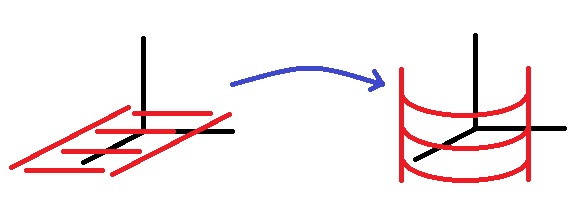
\includegraphics[width=0.60\textwidth]{C:/Users/Nacho/Documents/Latex/Facultad/GeometriaProyectiva/GeoProyectiva/enrollandoelcilindro.jpg}
	\caption{Enrollar una franja del plano en un cilindro es una isometría que no viene de un movimiento rígido.}
	\label{fig:enrollandoelcilindro}
\end{figure}
\end{obs}

Ahora que tenemos un poco más de idea de cómo es la geometría de una superficie, tratemos de precisar un poco la noción de geometría intrínseca. Una construcción que a cada superficie $S$ le asigna una función $\varphi_S:S\to\RR$ es un \textbf{invariante intrínseco} (con valores en $\RR$) si sólamente depende de la clase de isometría de $S$. Esto es, cada vez que $f:S\to S'$ es una isometría, vale que $\varphi_{S'}\circ f = \varphi_S$. Esta versión de invariantes intrínsecos depende únicamente de $S$, es decir, está libre de las coordenadas que podamos elegir sobre $S$. Para dar una versión en coordenadas, consideramos una construcción que a cada par $(S,\x)$ le asigna una función $\varphi_{S,\x}:\x(U)\to\RR$, donde $S$ es una superficie y $\x:U\to S$ una carta. Decimos en ese caso que una tal asignación es un \textbf{invariante intrínseco} si para cada isometría $f:S\to S'$ tenemos que $\varphi_{S',f\circ\x}\circ f = \varphi_{S,\x}$.

\begin{obs}
Las asignaciones $(S,\x)\stackrel{\varphi_{S,\x}}{\mapsto} (g_{ij}:\x(U)\to\RR)$ dadas por los coeficientes métricos son invariantes intrínsecos. En efecto, notemos primero que $f\circ\x$ es una carta de $S'$ (esto es simplemente usar que la composición de funciones diferenciables en el sentido de superficies es diferenciable, y eso es una fácil consecuencia de la Proposición ~\ref{prop::ensanchetecnico}). Ahora bien, queremos mirar los campos coordenados $(f\circ\x)_i$. Calculemos $(f\circ\x)_1$ la derivada respecto de la primera coordenada. Si tomamos $\alpha(t)=\x(u^1 +t,u^2)$ definida para $t\in(-\varepsilon,\varepsilon)$ tal que $(u^1+t,u^2)\in U$, entonces la derivada respecto de la primera coordenada de $f\circ\x$ en $u=(u^1,u^2)$ simplemente es $(f\circ\alpha)'(0)$. Si $p=\x(u)$, entonces $\alpha(0)=p$ y $\alpha'(0)=\x_1(p)$. Por lo tanto, por definición $(f\circ\alpha)'(0)=\diff_p f(\x_1(p))$. Hemos calculado entonces los campos coordenados de la carta $f\circ\x$ como $(f\circ\x)_i=\diff_p f(\x_i(p))$ (en particular, esto nos dice que los campos coordenados son intrínsecos). Entonces, sus coeficientes métricos están dados por $\varphi_{S',f\circ\x}\circ f(p)=\pint{\diff_p f(\x_i(p)),\diff_p f(\x_j(p))}$. Pero como $f$ es una isometría, $\diff_p f$ lo es, y así $\pint{\diff_p f(\x_i(p)),\diff_p f(\x_j(p))} = \pint{\x_i(p),\x_j(p)}$. Es decir, $\varphi_{S',f\circ\x}\circ f = \varphi_{S,\x}$. Esto prueba que los coeficientes métricos son intrínsecos.
\end{obs}

\begin{obs}
La métrica intrínseca $\diff_S:S\times S\to\RR$ es un invariante intrínseco. En efecto, esto se sigue de que si $f:S\to S'$ es una isometría y $\sigma:(a,b)\to S$ es una curva, entonces $f\circ\sigma:(a,b)\to S'$ es una curva que tiene igual longitud que $\sigma$. Para ver esto notemos que podemos escribir a la longitud de $\sigma$ en términos de $\mathrm{I}_p$ y como los coeficientes métricos son invariantes, la Primera Forma Fundamental debe serlo. Por lo tanto, la longitud se preserva por isometrías y así la distancia intrínseca es un invariante intrínseco como queríamos ver.
\end{obs}

\begin{defn}
Sea $S$ una superficie. Decimos que $\n:S\to\RR^3$ es un \textbf{campo normal} (o función de Gauss) si es diferenciable, $\norm{\n(p)}=1\;\forall p\in S$ y $\n(p)$ es ortogonal a $\mathrm{T}_p(S)$ para cada $p\in S$. 
\end{defn}

\begin{prop}
Sea $S\subseteq\RR^3$ una superficie y $p\in S$. Entonces, existe un abierto $V\subseteq S$ tal que $p\in V$ y $V$ posee un campo normal. Es decir, para cualquier superficie existen localmente campos normales.
\begin{proof}
Sea $\x:U\to S$ una carta con $\x(u)=p$. Tomemos la función $\n:\x(U)\to\RR^3$ dada por: $$\n(q)=\dfrac{\partial_1\x(\x^{-1}(q))\wedge\partial_2\x(\x^{-1}(q))}{\norm{\partial_1\x(\x^{-1}(q))\wedge\partial_2\x(\x^{-1}(q))}}$$ Notemos que $\n$ es diferenciable pues al componerla con la carta $\x$ obtenemos una función diferenciable (pues miramos $\partial_1\x$, $\partial_2\x$ son diferenciables y así su producto vectorial, y tomar norma también). Como cubrimos a $\x(U)$ sólo con la carta $\x$ y $\n\circ\x$ es diferenciable, en virtud de la Proposición ~\ref{prop::diferenciabilidadcartas} se sigue que $\n$ es diferenciable. Esto concluye la demostración.
\end{proof}
\end{prop}

\begin{prop}
Supongamos que $W\subseteq\RR^3$ es un abierto y $f:W\to\RR$ es de clase $\mathscr{C}^\infty$, $S=\{p\in\RR^3:f(p)=0\}$. Si $\nabla f(p)\neq 0$ para cada $p\in S$, entonces la superficie $S$ tiene un campo normal dado por $\n(p)=\dfrac{\nabla f(p)}{\norm{\nabla f(p)}}$.
\begin{proof}
El campo claramente es diferenciable, por ser $f$ de clase $\mathrm{C}^\infty$ y $\nabla f\neq 0$. Sea $X\in\mathrm{T}_p(S)$. Entonces, existe $\alpha:(-\varepsilon,\varepsilon)\to S$ tal que $\alpha(0)=p$ y $\alpha'(0)=X$. Ahora bien, como $\alpha((-\varepsilon,\varepsilon))\subseteq S$, tenemos que $f\circ\alpha\equiv 0$. Por lo tanto, por la regla de la cadena: $$0 = (f\circ\alpha)'(0)=\pint{\nabla f(\alpha(0)),\alpha'(0)} = \pint{\nabla f(p),X}$$ Es decir, $\nabla f(p)$ es ortogonal a $\mathrm{T}_p(S)$. Normalizándolo, se sigue lo deseado.
\end{proof}
\end{prop}

\begin{prop}
Si $S\subseteq\RR^3$ es una superficie conexa y existe $\n:S\to\RR^3$ campo normal, entonces hay exactamente dos campos: $\n$ y $-\n$.
\begin{proof}
Sea $\bd{m}:S\to\RR^3$ un campo normal. Como $\bd{m}(p),\n(p)\in(\mathrm{T}_p(S))^\perp$ y $\dim (\mathrm{T}_p)^\perp = 1$, debe existir $\lambda:S\to\RR$ tal que $\bd{m}(p)=\lambda(p)\n(p)$. Tomando norma, se sigue que $\abs{\lambda(p)}=1$ y así $\lambda:S\to \{-1,1\}$. Como $\lambda(p)=\pint{\bd{m}(p),\n(p)}$, $\lambda$ es continua y como $S$ es conexo, debe ser que $\lambda$ es constante. Esto nos dice que $\bd{m}(p)=\n(p)$ o $\bd{m}(p)=-\n(p)$. Como queríamos probar.
\end{proof}
\end{prop}

Sea $S\subseteq\RR^3$ es una superficie y $\n:S\to\RR^3$ es un campo normal. Si $p\in S$, y tenemos un vector tangente $X\in\mathrm{T}_p(S)$, entonces $X\n = (\n\circ\alpha)'(0)$ donde $\alpha:(-\varepsilon,\varepsilon)\to S$ con $\alpha(0)=p$ y $\alpha'(0)=X$. Como $\norm{\n\circ\alpha}=1$, tenemos que $\pint{(\n\circ\alpha)'(0),(\n\circ\alpha)(0)}=0$. Es decir, $\pint{X\n,\n}=0$. Esto implica que $X\n(p)\in \langle\n(p)\rangle^\perp = \mathrm{T}_p(S)$. Es decir, tenemos una asignación $\diff_p\n:\mathrm{T}_p(S)\to\mathrm{T}_p(S)$ dada por $\diff_p\n(X)=X\n(p)$.

\begin{defn}
Sea $S$ una superficie y $\n:S\to\RR^3$ un campo normal. Si $p\in S$, entonces $L_p=-\diff_p\n:\mathrm{T}_p(S)\to\mathrm{T}_p(S)$, $L_p(X)=-\diff_p\n(X) = -X\n(p)$ se denomina el \textbf{operador de forma} de $S$ en $p$.
\end{defn}

El operador de forma nos está midiendo la geometría de todas las curvas sobre $S$ que pasan por $p$ juntas. El problema de no tener una base distinguida para $\mathrm{T}_p(S)$ lo resolveremos mirando los autovectores del operador de forma $L$. En particular, forman una base ortonormal en virtud de la siguiente proposición:

\begin{prop}
Sea $S\subseteq\RR^3$ una superficie. Su operador de forma $L_p$ es autoadjunto para cada $p\in S$. En particular, $L_p$ es diagonalizable, con autovalores reales y una base ortonormal de autovectores.
\begin{proof}
Sea $\x:U\to S$ una carta con $\x(u)=p$. Notemos que $\pint{\n(p),\x_i(p)}=0$ por ser $\n(p)$ ortogonal al tangente $\mathrm{T}_p(S)$ y $\{\x_1(p),\x_2(p)\}$ una base del espacio tangente. Derivando la función $f(q)=\pint{\n(q),\x_i(q)}$ respecto de $\x_j(p)$ tenemos que: $$0 = \x_j(p)\pint{\n(p),\x_i(p)} = \pint{\x_j(p)\n(p),\x_i(p)} + \pint{\n(p),\x_j(p)\x_i(p)}$$ Ahora bien, $\x_j\x_i=\partial_j\x_i=\partial_j\partial_i\x$. Como $\x$ es de clase $\mathscr{C}^\infty$, las derivadas cruzadas conmutan, y así $\partial_j\partial_i\x = \partial_i\partial_j\x$. Por lo tanto, $\pint{\x_j(p)\n(p),\x_i(p)} = \pint{\x_i(p)\n(p),\x_j(p)}$. Es decir, $\pint{\diff_p(\x_j),\x_i} = \pint{\x_j,\diff_p(\x_i)}$. Como $\{\x_1(p),\x_2(p)\}$ es una base de $\mathrm{T}_p(S)$, esto concluye la demostración.
\end{proof}
\end{prop}

Notemos que la demostración anterior funciona principalmente por el hecho de que las derivadas cruzadas conmutan. Es decir, que para los campos coordenados $\x_i,\x_j$ tenemos que $\diff\x_i(\x_j) - \diff\x_j(\x_i)=0$. Ahora bien, un \textbf{campo tangente} a una superficie $S$ es una función $\X:S\to\RR^3$ tal que para cada $p\in S$ se tiene $\X(p)\in\mathrm{T}_p(S)$. Denotamos por $\mathfrak{X}(S)$ al conjunto de todos los campos tangentes a $S$ que son diferenciables. Si tenemos $X,Y\in\mathfrak{X}(S)$, por lo general no es cierto que las derivadas cruzadas conmuten. Es decir, derivando a $Y$ respecto de $X(p)$ y a $X$ respecto de $Y(p)$ obtenemos resultados distintos. El \textbf{corchete de Lie} mide precisamente esto: $[X,Y]_p=X(p)Y-Y(p)X$.

\begin{defn}
Sea $S\subseteq\RR^3$ una superficie y $p\in S$. La \textbf{curvatura Gaussiana} de $S$ en $p$ se define por $\kappa(p)=\det L_p$ y la \textbf{curvatura media} de $S$ en $p$ se define por $H(p)=\dfrac{1}{2}\tr L_p$. Las \textbf{curvaturas principales} de $S$ en $p$ son los autovalores de $L_p$ y las direcciones correspondientes a los autovectores son las \textbf{direcciones principales}. Por último, decimos que $p\in S$ es un punto \textbf{plano} si $\kappa(p)=0$, es \textbf{umbílico} si las dos curvaturas principales son iguales, es \textbf{elíptico} si $\kappa(p)>0$ y es \textbf{hiperbólico} si $\kappa(p)<0$. \textcolor{red}{Agregar dibujo}
\end{defn}

Sea $\x:U\to S$ una carta y sea $p\in\x(U)$. Como $\{\x_1(p),\x_2(p)\}$ es una base del espacio tangente $\mathrm{T}_p(S)$, existen escalares $L^i_{\; j}(p)$ tales que $L_p(\x_j(p))=\displaystyle\sum_{i=1}^2 L^i_{\; j}(p) \x_i(p)$. Esto define funciones $L^i_{\; j}:\x(U)\to\RR$. Como $\x_\ell\in\mathrm{T}_p(S)$, la función $\pint{\n,\x_\ell}$ es idénticamente nula. Derivándola respecto de $\x_j(p)$ para cada $p$ y usando la regla del producto, obtenemos $\pint{\diff_p\n(\x_j(p)),\x_\ell(p)}+\pint{\n(p),\diff_p\x_\ell(\x_j(p))} = 0$. Por lo tanto, se sigue que: $$\pint{L_p(\x_j(p)),\x_\ell(p)} = \pint{\n(p),\diff_p\x_\ell(\x_j(p))}$$ Esto implica que $\displaystyle\sum_{k=1}^2 L^k_{\; j}(p)\pint{\x_k(p),\x_\ell(p)} = \pint{\n(p),\diff_p\x_\ell(\x_j(p))}$. Pero en término de los coeficientes métricos, esto es $\displaystyle\sum_{k=1}^2 L^k_{\; j}(p) g_{k\ell}(p) = \pint{\n(p),\diff_p\x_\ell(\x_j(p))}$. Si multiplicamos a ambos lados por $g^{\ell i}(p)$ y sumamos respecto de $\ell$, obtenemos que: $$\displaystyle\sum_{\ell=1}^2 \sum_{k=1}^2 L^k_{\; j}(p)g_{k\ell}(p)g^{\ell i}(p) = \sum_{k=1}^2 L^k_{\; j}(p)\left(\sum_{\ell=1}^2 g_{k\ell}(p)g^{\ell i}(p)\right) = \sum_{k=1}^2 L^k_{\; j}(p) \delta_{i}^k = L^i_{\;j}(p)$$ Es decir, pudimos obtener el despeje: \begin{eqnarray}\label{eq::ecestructura}L^i_{\;j}(p) = \displaystyle\sum_{\ell=1}^2 \pint{\n(p),\diff_p\x_\ell(\x_j(p))}g^{\ell i}(p)\end{eqnarray} En particular, las funciones $L^i_{\;j}$ son diferenciables por ser sumas y productos de funciones diferenciables. Ahora bien, si miramos al operador de forma $L_p$ en la base ${\mathscr{B}(p)=\{\x_1(p),\x_2(p)\}}$, su matriz asociada es $[L_p]_{\mathscr{B}(p)}=\begin{pmatrix}L^1_{\;1}&L^1_{\;2}\\ L^2_{\; 1}& L^2_{\; 2}\end{pmatrix}$. Como la curvatura Gaussiana de $S$ en $p$ es $\kappa(p)=\det L_p = \det [L_p]_{\mathscr{B}(p)} = L^1_{\;1}L^{2}_{\;2}-L^{1}_{\;2}L^2_{\;1}$, que resulta diferenciable por serlo las funciones $L^{i}_{\;j}$. De manera análoga, la curvatura media de $S$ en $p$ es $H(p)=\dfrac{1}{2}\tr L_p =\dfrac{1}{2}\tr [L_p]_{\mathscr{B}(p)} =\dfrac{1}{2}\left(L^1_{\;1} + L^2_{\; 2}\right)$, que también resulta diferenciable.

Supongamos que las curvaturas principales de $S$ en $p$ son $\kappa_1(p)\leq \kappa_2(p)$. Sabemos que son las raíces del polinomio característico $x^2 - \tr L_p x + \det L_p = x^2 - 2H(p)x + \kappa(p)$. Es decir, $\kappa_1 = H(p)-\sqrt{H(p)^2 - \kappa(p)}$ y $\kappa_2(p)=H(p)+\sqrt{H(p)^2 - \kappa(p)}$. Notemos que $\kappa_1$ y $\kappa_2$ son diferenciables siempre y cuando esa raíz sea no nula (pues sería suma y composición de funciones diferenciables). Pero esto implica que son diferenciables siempre y cuando las raices sean distintas, y en nuestro lenguaje geométrico eso es que el punto $p$ no sea umbilical. Por otra parte, si $p$ no es umbilical, hay un entorno $\x(U)$ de $p$ tal que ningún punto es umbilical (esto es por la continuidad de $\kappa_1-\kappa_2$ que no se anula en $p$). Podemos probar entonces el siguiente resultado.
\begin{prop}
Sea $S\subseteq\RR^3$ una superficie y $p\in S$. Si $p$ no es un punto umbilical, existe un entorno de $p$ donde podemos definir un campo tangente unitario con la dirección principal de cada autovector.
\begin{proof}
\textcolor{red}{Ejercicio!} (Usar Implícita?)
\end{proof}
\end{prop}

Fijemos una carta $\x:U\to S$. Todo lo que hagamos ahora dependerá de esta carta, pero veremos que podemos pasar bien de una carta a la otra. Sabemos que $\{\x_1(p),\x_2(p),\n(p)\}$ es una base de $\RR^3$. Además, podemos escribir: $$\begin{cases}\diff_p\n(\x_j(p)) = -L_p(\x_j(p)) = -\displaystyle\sum_{i=1}^2 L^i_{\;j}(p)\x_i(p)\\ \diff_p\x_i(\x_j(p)) = \displaystyle\sum_{k=1}^2 \Gamma_{ij}^{\;\;k}(p)\x_k(p) + L_{ij}(p)\n(p)\end{cases}$$ Estas son las denominadas \textbf{ecuaciones de estructura}. Ahora bien, como las derivadas cruzadas conmutan $\diff_p\x_i(\x_j(p))=\diff_p\x_j(\x_i(p))$, tenemos que $\Gamma_{ij}^{\;\;k}=\Gamma_{ji}^{\;\;k}$ y $L_{ij}=L_{ji}$. Esta relación de (anti)simetría que aparece entre los coeficientes y las ecuaciones de estructura vendría a generalizar en algún sentido a la antisimetría de las ecuaciones de Frenet-Serret en curvas. Ahora bien, como $\n(p)$ es ortogonal a $\x_1(p)$ y $\x_2(p)$, es claro que tenemos $L_{ij}=\pint{\diff_p\x_i(\x_j(p)),\n(p)}$. Por lo tanto, la ecuación ~\ref{eq::ecestructura} se puede reescribir como $L^i_{\; j}(p)=\displaystyle\sum_{\ell=1}^2 L_{\ell j}(p)g^{\ell i}$. De manera similar a lo que venimos haciendo tenemos que $\pint{\diff_p\x_i(\x_j(p)),\x_\ell(p)} = \displaystyle\sum_{k=1}^2 \Gamma_{ij}^{\;\;k}(p)\pint{\x_k(p),\x_\ell(p)}=\displaystyle\sum_{k=1}^2\Gamma_{ij}^{\;\;k}(p)g_{k\ell}(p)$. Por lo tanto, multiplicando por $g^{\ell r}(p)$ y sumando sobre $\ell$, obtenemos que: $$\displaystyle\sum_{\ell=1}^2 \pint{\diff_p\x_i(\x_j(p)),\x_\ell(p)}g^{\ell r} = \sum_{\ell=1}^2 \sum_{k=1}^2 \Gamma_{ij}^{\;\; k}(p)g_{k\ell}(p)g^{\ell r}(p) = \sum_{k=1}^2 \Gamma_{ij}^{\;\; k}(p)\delta_{r}^k = \Gamma_{ij}^{\;\;r}(p)$$ A los coeficientes $\Gamma_{ij}^{\;\;k}$ se los denomina \textbf{símbolos de Christoffel}. Veamos que son de naturaleza intrínseca. Es decir, podemos escribirlos sólo en términos de los coeficientes métricos y la carta.

\begin{prop}
Para todos $i,j,k$, podemos expresar a los símbolos de Christoffel de manera intrínseca: $$\Gamma_{ij}^{\;\;k}(p)=\dfrac{1}{2}\displaystyle\sum_{\ell=1}^2 g^{\ell k}(p)\left(\x_j(p) g_{i\ell}(p)-\x_\ell(p) g_{ij}(p)+\x_i(p) g_{ij}(p)\right)$$
\begin{proof}
Simplemente es usar la regla del producto para derivar al producto interno: $$\x_j(p) g_{i\ell}(p) = \x_j(p)\pint{\x_i(p),\x_\ell(p)} = \pint{\diff_p\x_i(\x_j(p)),\x_\ell(p)}+\pint{\x_i(p),\diff_p\x_\ell(\x_j(p))}$$ Procediendo de manera análoga, obtenemos: \begin{align*}\x_\ell(p) g_{ij}(p)&= \pint{\diff_p\x_i(\x_\ell(p)),\x_j(p)}+\pint{\x_i(p),\diff_p\x_j(\x_\ell(p))} \\ \x_i(p) g_{j\ell}(p)&= \pint{\diff_p\x_j(\x_i(p)),\x_\ell(p)}+\pint{\x_j(p),\diff_p\x_\ell(\x_i(p))}\end{align*} Sumando alternadamente estas tres identidades, se tiene: $$\x_j(p) g_{i\ell}(p)-\x_\ell(p) g_{ij}(p)+\x_i(p) g_{ij}(p) = 2\pint{\diff_p\x_i(\x_j(p)),\x_\ell(p)}$$ Multiplicando por $g^{\ell k}(p)$ y sumando sobre $\ell$ se sigue lo deseado.
\end{proof}
\end{prop}

Para concluir esta sección, vamos a probar que la curvatura gaussiana de una superficie es intrínseca. Esto se seguirá fácilmente de las ecuaciones de Gauss y Codazzi-Mainardi. En esta parte usaremos la convención de suma de Einstein. De acuerdo a esta convención, cuando un índice aparece arriba y abajo entonces se lleva a cabo una suma respecto de ese índice. Por ejemplo, en vez de escribir $X=X^1\x_1(p)+X^2\x_2(p)$, con esta convención escribiremos $X=X^i\x_i(p)$. Otro ejemplo sería la ecuación intrínseca de los símbolos de Christoffel $\Gamma_{ij}^{\;\;k}(p)=\dfrac{1}{2} g^{\ell k}(p)\left(\x_j(p) g_{i\ell}(p)-\x_\ell(p) g_{ij}(p)+\x_i(p) g_{ij}(p)\right)$. Como se ve, ya usamos esta convención colocando los índices en los lugares correctos, sólo que escribíamos la suma.

\begin{defn}
Sea $S\subseteq\RR^3$ una superficie, $\x:U\to S$ una carta. Los coeficientes del \textbf{tensor de curvatura} se definen por $$R_{i\; jk}^{\;\ell} = \x_j\Gamma_{ij}^{\;\;\ell} - \x_k\Gamma_{ik}^{\;\;\ell}+ \Gamma_{ik}^{\;\; p}\Gamma_{pj}^{\;\;\ell}-\Gamma_{ij}^{\;\; p}\Gamma_{pk}^{\;\;\ell}$$
donde en esa ecuación usamos la convención de suma. Notar que los coeficientes del tensor de curvatura son intrínsecos por serlo los símbolos de Christoffel.
\end{defn}

\begin{prop}
Sobre una superficie $S\subseteq\RR^3$ tenemos las dos siguientes ecuaciones:

\begin{align}
R_{i\; jk}^{\;\ell} &= L_{ik} L^{\ell}_{\; j} - L_{ij}L^{\ell}_{\; k} \tag{Gauss} \\
\partial_k L_{ij}-\partial_j L_{ik} &= \Gamma_{ik}^{\;\;\ell} L_{\ell j} - \Gamma_{ij}^{\;\;\ell} L_{\ell k} \tag{Codazzi-Mainardi}
\end{align}
\begin{proof}
Recordemos que $\partial_j\x_i = L_{ij}\n + \Gamma_{ij}^{\;\;\ell}\x_\ell$ y $\partial_k\n = L^{\ell}_{\; k}\x_\ell$. Por lo tanto, mirando la derivada parcial respecto de la $k$-ésima dirección, se tiene que: \begin{align*}\partial_k\partial_j \x_i &= \partial_k L_{ij}\n + L_{ij}\partial_k\n + \partial_k\Gamma_{ij}^{\;\;\ell} \; \x_\ell + \Gamma_{ij}^{\;\;\ell}\partial_k\x_\ell \\ &= \partial_k L_{ij} \n + L_{ij}L^{\ell}_{\; k}\x_\ell + \partial_k\Gamma_{ij}^{\;\; \ell}\x_\ell + \Gamma_{ij}^{\;\;\ell}(L_{\ell k}\n + \Gamma_{\ell k}^{\;\; m}\x_m) \\ &= \left(\partial_k L_{ij} + \Gamma_{ij}^{\;\;\ell} L_{\ell k}\right)\n + \left( L_{ij}L^\ell_{\; k}+\partial_k\Gamma_{ij}^{\;\;\ell}\right)\x_\ell + \Gamma_{ij}^{\;\;\ell}\Gamma_{\ell k}^{\;\; m}\x_m\\ &= \left(\partial_k L_{ij} + \Gamma_{ij}^{\;\;\ell} L_{\ell k}\right)\n + \left( L_{ij}L^\ell_{\; k}+\partial_k\Gamma_{ij}^{\;\;\ell}\right)\x_\ell + \Gamma_{ij}^{\;\; m}\Gamma_{m k}^{\;\; \ell}\x_\ell \\ &= \left(\partial_k L_{ij} + \Gamma_{ij}^{\;\;\ell} L_{\ell k}\right)\n + \left( L_{ij}L^\ell_{\; k}+\partial_k\Gamma_{ij}^{\;\;\ell} + \Gamma_{ij}^{\;\; m}\Gamma_{mk}^{\;\;\ell}\right)\x_\ell\end{align*} Ahora bien, como las derivadas cruzadas $\partial_k\partial_j\x_i = \partial_j\partial_k\x_i$ conmutan, igualando las componentes obtenemos las siguientes dos ecuaciones:
$$\begin{cases} \partial_k L_{ij} + \Gamma_{ij}^{\;\;\ell}L_{\ell k} = \partial_j L_{ik} + \Gamma_{ik}^{\;\;\ell}L_{\ell j}\\   L_{ij}L^\ell_{\; k}+\partial_k\Gamma_{ij}^{\;\;\ell} + \Gamma_{ij}^{\;\; m}\Gamma_{mk}^{\;\;\ell}= L_{ik}L^\ell_{\; j}+\partial_j\Gamma_{ik}^{\;\;\ell} + \Gamma_{ik}^{\;\; m}\Gamma_{mj}^{\;\;\ell}\end{cases}$$ Si pasamos restando los términos obvios en cada ecuación, de la primera obtenemos la ecuación de Gauss y en la segunda la de Codazzi-Mainardi. Y estamos.
\end{proof}
\end{prop}

Estamos en condiciones de probar:

\begin{teo}[Egregium]
La curvatura gaussiana $\kappa$ es intrínseca a la superficie.
\begin{proof}
Por la ecuación de Gauss, $R_{i\; jk}^{\;\ell} = L_{ik}L^{\ell}_{\; j} - L_{ij}L^{\ell}_{\; k}$. Notemos que $$R_{i\; jk}^{\;\ell}g_{\ell m} = L_{ik}L^{\ell}_{\; j}g_{\ell m} - L_{ij}L^{\ell}_{\; k}g_{\ell m} = L_{ik}L_{mj}-L_{ij}L_{mk}$$ Para $i=k=1$, $j=m=2$ resulta que $R_{1\; 21}^{\; \ell}g_{\ell 2} = L_{11}L_{22}-L_{12}L_{21} = \det (L_{ij})_{1\leq i,j\leq 2}$. Pero $(L_{ij})_{1\leq i,j\leq 2} = (L^{i}_{\; j})_{1\leq i,j\leq 2}\cdot (g_{ij})_{1\leq i,j\leq 2}$ y así $\kappa = \dfrac{1}{g}R_{1\; 21}^{\;\ell}g_{\ell 2}$. Esto concluye la demostración.
\end{proof}
\end{teo}

\section{Curvas sobre una Superficie}

El objetivo será tratar de usar las cosas que sabemos sobre las curvas para caracterizar a la superficie. Sea $S\subseteq\RR^3$ una superficie y $\sigma:(a,b)\to\RR^3$ una curva parametrizada por longitud de arco tal que $\sigma(s)\in S$ para todo $s\in (a,b)$. En el caso de las curvas planas sabíamos que la curvatura tenía más información: el signo. Moralmente, una superficie no es más que un plano deformado, así que si tenemos una curva dentro de una superficie la situación debería ser análoga a una curva plana. En este caso, las curvas planas tienen un signo porque dada la tangente $\T(s)$ hay una manera natural de completarlo a una base de $\RR^2$. Para una curva contenida en una superficie, tenemos la tangente $\T(s)$ y el campo normal $\n(\sigma(s))$. Estas dos direcciones son ortogonales, pues $\T(s)$ es la velocidad de una curva y así $\T(s)\in\mathrm{T}_{\sigma(s)}S$. Ahora sí tenemos una elección canónica para un vector $\M(s)$ para completar a una base ortonormal orientada. Sólo debemos tomar $\M(s)=\n(\sigma(s))\wedge\T(s)$. A esta elección de normal a la curva la denominamos la \textbf{norma intrínseca} de $\sigma$ en $S$.

Ahora bien, como $\{\T(s),\M(s),\n(\sigma(s))\}$ forma una base ortonormal orientada, podemos escribir a $\T'(s)$ en esa base. Como $\norm{\T(s)}^2=1$ para todo $s$, derivando el producto interno $\pint{\T(s),\T(s)}$ se obtiene que $\pint{\T(s),\T'(s)}=0$. Entonces, tenemos que $\T'(s)=\kappa_g(s)\M(s) + \kappa_n(s)\n(\sigma(s))$. A $\kappa_g$ la llamamos la \textbf{curvatura geodésica} mientras que a $\kappa_n$ la llamamos la \textbf{curvatura normal}. Notemos que, por el Teorema de Pitágoras, $\kappa(s)=\norm{\T'(s)} = \sqrt{\kappa_g^2(s) + \kappa_n^2(s)}$. 

Supongamos que $\x:U\to S$ es una carta y que la traza de $\sigma$ está contenida en la traza de la carta. Es decir, $\sigma((a,b))\subseteq\x(U)$. Sean $\sigma^1,\sigma^2:(a,b)\to\RR$ funciones tales que $\x^{-1}(\sigma(s))=(\sigma^1(s),\sigma^2(s))$ (esto podemos hacerlo por el clásico argumento de ensanchar con la Proposición ~\ref{prop::ensanchetecnico}). Las funciones $\sigma^1,\sigma^2$ resultan diferenciables y se denominan las \textbf{funciones coordenadas} de la curva. Es decir, $\sigma(s)=\x(\sigma^1(s),\sigma^2(s))$. Derivando y usando la regla de la cadena, $\sigma'(s)=\displaystyle\sum_{i=1}^2 \partial_i\x(\sigma^1(s),\sigma^2(s))(\sigma^i)'(s) = \displaystyle\sum_{i=1}^2 (\sigma^i)'(s)\x_i(\sigma(s))$. Notemos que $\left.\dfrac{\diff}{\diff s}\right\rvert_{s=s_0} \x_i(\sigma(s)) = \diff_{\sigma(s_0)}\x_i(\sigma'(s_0))$. Usando esto y la regla de la cadena, podemos volver a derivar y así $\sigma''(s)=\displaystyle\sum_{i=1}^2 (\sigma^i)''(s)\x_i(\sigma(s)) + \displaystyle\sum_{i,j=1}^2 (\sigma^j)'(s)(\sigma^i)'(s) \diff_{\sigma(s)}\x_i(\x_j(\sigma(s)))$. Recordando que $\diff_p \x_i(\x_j(p)) = \displaystyle\sum_{k=1}^2 \Gamma_{ij}^{\;\;k}(p)\x_k(p) + L_{ij}(p)\n(p)$ y manipulando la suma, obtenemos que: $$\sigma''=\left(\displaystyle\sum_{i,j=1}^2 (\sigma^i)'(\sigma^j)'L_{ij}\right)\n + \displaystyle\sum_{k=1}^2 \left((\sigma^k)'' + \displaystyle\sum_{i,j=1}^2 \Gamma_{ij}^{\;\;k}(\sigma^i)'(\sigma^j)'\right)\x_k$$ donde cada función está evaluada en el único lugar que podría estarlo. Esto implica que: $$\kappa_n = \displaystyle\sum_{i,j=1}^2 (\sigma^i)'(\sigma^j)'L_{ij} = \displaystyle\sum_{i,j,\ell=1}^2 (\sigma^i)'(\sigma^j)'L^{\ell}_{\;j}g_{\ell i} = \pint{L\sigma',\sigma'}$$ Esto nos motiva a considerar la forma cuadrática $\mathrm{II}_p(X,Y)=\pint{LX,Y}$, que llamaremos la \textbf{Segunda Forma Fundamental}. Notemos que la curvatura normal $\kappa_n$ sólo depende de la velocidad en el punto. Es decir, la curvatura normal no ve la aceleración y por lo tanto toda esa información está contenida en la curvatura geodésica.

\begin{prop}
La curvatura geodésica de una curva en una superficie $S\subseteq\RR^3$ es intrínseca.
\begin{proof}
Ya vimos que si $\sigma$ es una curva sobre $S$ parametrizada por longitud de arco entonces podemos escribir a $\T'(s)=\sigma''(s)$ en términos de la base $\{\x_1(s),\x_2(s),\n(\sigma(s))\}$ como: $$\sigma''=\left(\displaystyle\sum_{i,j=1}^2 (\sigma^i)'(\sigma^j)'L_{ij}\right)\n + \displaystyle\sum_{k=1}^2 \left((\sigma^k)'' + \displaystyle\sum_{i,j=1}^2 \Gamma_{ij}^{\;\;k}(\sigma^i)'(\sigma^j)'\right)\x_k$$ Como las direcciones $\x_1(s),\x_2(s)$ son ortogonales a $\n(s)$, debemos tener que: $$\kappa_g(s)\M(s) = \displaystyle\sum_{k=1}^2\left( (\sigma^k)''(s) + \displaystyle\sum_{i,j=1}^2 \Gamma_{ij}^{\;\;k}(\sigma(s)) (\sigma^i)'(s)(\sigma^j)'(s)\right)\x_k(s)$$ Ahora bien, tenemos que $\kappa_g(s)=\pint{\kappa_g(s)\M(s),\M(s)} = \pint{\kappa_g(s)\M(s),\n(\sigma(s))\wedge\T(s)}$. Recordando que $\pint{u,v\wedge w} = \det\begin{pmatrix} | & | & | \\ u & v & w \\ | & | & | \end{pmatrix}:=[u|v|w]$, obtenemos la fórmula $$\kappa_g(s)=\displaystyle\sum_{k=1}^2 \left( (\sigma^k)''(s) + \displaystyle\sum_{i,j=1}^2 \Gamma_{ij}^{\;\;k}(\sigma(s)) (\sigma^i)'(s)(\sigma^j)'(s)\right) [\x_k(s)|\n(\sigma(s))|\T(s)]$$
Por otra parte, si $\varepsilon_{ij}(s)=\det[\n(\sigma(s))|\x_i(s)|\x_j(s)]$, entonces $\varepsilon_{12}(s)=-\varepsilon_{21}(s)=g(s)$, donde $g$ es el determinante de la matriz asociada a la Primera Forma Fundamental, y $\varepsilon_{11}=\varepsilon_{22}=0$. Esto nos dice que $\varepsilon$ es intrínseco, pues los coeficientes métricos lo son. Como podemos escribir $\T(s)=\sigma'(s)=\displaystyle\sum_{\ell=1}^2 (\sigma^\ell)'(s)\x_{\ell}(\sigma(s))$, se tiene que: \begin{align*}\kappa_g(s)&=\displaystyle\sum_{\ell=1}^2 \left((\sigma^k)''(s) + \displaystyle\sum_{i,j=1}^2 \Gamma_{ij}^{\;\;k}(\sigma(s)) (\sigma^i)'(s)(\sigma^j)'(s)\right)(\sigma^\ell)'(s)[\x_k(s),\n(\sigma(s),\x_\ell(s)]\\&=\displaystyle\sum_{\ell=1}^2 \left((\sigma^k)''(s) + \displaystyle\sum_{i,j=1}^2 \Gamma_{ij}^{\;\;k}(\sigma(s)) (\sigma^i)'(s)(\sigma^j)'(s)\right)(\sigma^\ell)'(s)\varepsilon_{\ell k}(s)\end{align*} Por lo tanto, expresamos a $\kappa_g(s)$ en términos de cosas intrínsecas, debe ser intrínseco. Como queríamos probar.
\end{proof}
\end{prop}

Si bien la curvatura geodésica es intrínseca, en general las expresiones intrínsecas son complicadas. Veamos una fórmula extrínseca para la curvatura geodésica que, en términos calculatorios, es mucho más simple y útil.

\begin{prop}\label{prop::curvaturageodesicaextrinseca}
Si $S\subseteq\RR^3$ es una superficie y $\sigma:(a,b)\to S$ es una curva sobre $S$, entonces $$\kappa_g(s)=\kappa(s)\pint{\n(\sigma(s)),\B(s)}$$ donde $\kappa$ es la curvatura de $\sigma$ y $\B$ su vector binormal.
\begin{proof}
Como $\T'(s)=\kappa_g(s)\M(s)+\kappa_n(s)\n(\sigma)$ y $\pint{\n(\sigma(s)),\M(s)}=0$, tenemos que $\kappa_g(s)=\pint{\T'(s),\M(s)}$. Ahora bien, notemos que: \begin{align*}\pint{\T'(s),\M(s)}&=\pint{\T'(s),\n(\sigma(s))\wedge\T(s)}\\&=[\T'(s)|\n(\sigma(s))|\T(s)]\\&=[\n(\sigma(s))|\T(s)|\T'(s)] \\&= \pint{\n(\sigma(s)),\T(s)\wedge\T'(s)} \\&= \kappa(s)\pint{\n(\sigma(s)),\T(s)\wedge\N(s)}\\&=\kappa(s)\pint{\n(\sigma(s)),\B(s)}\end{align*} Esto concluye la demostración.
\end{proof}
\end{prop}

Ya dijimos que moralmente la situación de una superficie debería ser como la del plano. Queremos definir el análogo a una recta dentro de una superficie. Para esto, queremos que no esté curvada \textit{intrínsecamente}. Como la parte intrínseca de la curvatura es la geodésica, podríamos pensar que una curva es recta dentro de la superficie si su curvatura geodésica es $0$. Es decir, si solo se deforma como la superficie, en la dirección de la normal. Esto motiva la siguiente definición:

\begin{defn}
Una curva $\sigma:(a,b)\to S$ parametrizada por longitud de arco en una superficie $S\subseteq\RR^3$ es una \textbf{geodésica} si su curvatura geodésica es nula.
\end{defn}

\begin{prop}
Una curva $\sigma$ en $S$ es una geodésica si y sólo si $[\n(\sigma(s))|\T(s)|\T'(s)]=0$.
\begin{proof}
Esto es claro, pues siguiendo la demostración de la Proposición ~\ref{prop::curvaturageodesicaextrinseca} tenemos que $\kappa_g(s)=[\n(\sigma(s))|\T(s)|\T'(s)]$.
\end{proof}
\end{prop}

\begin{obs}
Lo que nos dice la Proposición anterior es que una curva es geodésica si y sólo si la normal a la curva $\N$ es paralela a la normal a la superficie $\n$. Es decir, la superficie \textbf{no} ve la forma en la que cambia la tangente, que en parte fue lo que nos motivó a definir las geodésicas así.
\end{obs}

\begin{ex}\textcolor{red}{Dibujar esto y demostrarlo!}
En la esfera $S^2$ los \textbf{círculos máximos} (intersecciones de planos que pasan por el origen con $S^2$) son geodésicas.

Si una superficie $S$ tiene un plano de simetría $\Pi$, entonces la curva $\Pi\cap S$ es una geodésica.

Si $S$ es una \textbf{superficie de revolución}, entonces los círculos de los puntos críticos son geodésicas.

Si $R\subseteq S$ es una recta contenida en $S$, entonces $R$ es una geodésica. Por ejemplo, en un hiperboloide de una hoja.
\end{ex}

\begin{prop}
Ser geodésica es una propiedad intrínseca de la curva.
\begin{proof}
Sea $\sigma:(a,b)\to S$ una geodésica y $f:S\to S'$ una isometría. Veamos que $f\circ\sigma$ es una geodésica. En efecto, $f\circ\sigma$ está parametrizada por longitud de arco, pues la longitud de las curvas se preserva por isometrías (ya que depende de la Primera Forma Fundamental que es intrínseca). Por otra parte, su curvatura geodésica es la misma que la de $\sigma$ por ser la curvatura geodésica intrínseca. Por lo tanto, $f\circ\sigma$ es una curva parametrizada por longitud de arco con curvatura geodésica nula. Esto implica que $f\circ\sigma$ es una geodésica.
\end{proof}
\end{prop}

\begin{prop}
Sea $S\subseteq\RR^3$ una superficie, y sean $p\in S$ un punto, $X\in\mathrm{T}_pS$ un vector tangente unitario. Entonces existen $\varepsilon>0$ y $\sigma:(-\varepsilon,\varepsilon)\to S$ tal que $\sigma(0)=p$, $\sigma'(0)=X$ y $\sigma$ es una geodésica. Más aún, si $\sigma:(a,b)\to S$, $\tau:(c,d)\to S$ son dos geodésicas con $0\in (a,b)\cap (c,d)$ y $\sigma(0)=\tau(0)=p$, $\sigma'(0)=\tau'(0)=X$, entonces existe $\varepsilon>0$ tal que $(-\varepsilon,\varepsilon)\subseteq (a,b)\cap (c,d)$ y $\left.\sigma\right\rvert_{(-\varepsilon,\varepsilon)}=\left.\tau\right\rvert_{(-\varepsilon,\varepsilon)}$.
\begin{proof}
Sea $\x:U\to S$ una carta tal que $p\in\x(U)$ y sea $u_0\in U$ tal que $\x(u_0)=p$. Escribamos $X=\displaystyle\sum_{i=1}^2 X^i \x_i(p)$. Sabemos que dada una curva $\sigma:(a,b)\to \x(U)$, existen funciones $\sigma^1,\sigma^2:(a,b)\to\RR$ tales que $\sigma(s)=\x(\sigma^1(s),\sigma^2(s))$. Es decir, toda curva contenida en la imagen de una carta viene de la imagen de una curva en $U$. Consideremos el siguiente Problema de Valores Iniciales: $$\begin{cases}(\sigma^k)''(s) + \displaystyle\sum_{i,j=1}^2 \Gamma_{ij}^{\;\;k}(\x(\sigma^1(s),\sigma^2(s))(\sigma^i)(s)(\sigma^j)(s) &= 0 \text{ si }k=1,2\\ \sigma^i(0)&=u_0^i \text{ si }i=1,2\\ (\sigma^i)'(0)&=X^i \text{ si }i=1,2\end{cases}$$ La primera condición está dada para que $\kappa_g$ sea idénticamente nula, la segunda condición para que $\sigma(0)=\x(\sigma^1(0),\sigma^2(0)) = p$ y la tercera para que $\sigma'(0)=\displaystyle\sum_{i=1}^2 X^i \x_i(p)=X$. Por el Teorema de Existencia y Unicidad para Ecuaciones Diferenciales Ordinarias, existen funciones $\sigma^1,\sigma^2:(-\varepsilon,\varepsilon)\to\RR$ que resuelven el Problema de Valores Iniciales. Podemos tomar $\varepsilon$ suficientemente chico como para que $(\sigma^1(t),\sigma^2(t))\in U$ para todo $t\in(-\varepsilon,\varepsilon)$ por ser $\sigma^1,\sigma^2$ continuas y $U$ abierto. Consideremos entonces $\sigma:(-\varepsilon,\varepsilon)\to S$ dada por $\sigma(s)=\x(\sigma^1(s),\sigma^2(s))$. Veamos que $\sigma$ es una geodésica. Para ello, debemos probar que $\sigma$ está parametrizada por longitud de arco. Es decir, $\norm{\sigma'(s)}=1$ para todo $s$. Recordemos que, derivando y usando la regla de la cadena y un par de identidades, se tiene que: $$\sigma''=\left(\displaystyle\sum_{i,j=1}^2 (\sigma^i)'(\sigma^j)'L_{ij}\right)\n + \displaystyle\sum_{k=1}^2 \left((\sigma^k)'' + \displaystyle\sum_{i,j=1}^2 \Gamma_{ij}^{\;\;k}(\sigma^i)'(\sigma^j)'\right)\x_k$$ Como $\sigma^1,\sigma^2$ resuelven el Problema de Valores Iniciales, los términos que acompañan a $\x_k$ se desvanecen, y así en nuestro caso tenemos que: $$\sigma''(s)=\left(\displaystyle\sum_{i,j=1}^2 (\sigma^i)'(s)(\sigma^j)'(s)L_{ij}(\sigma(s))\right)\n(\sigma(s))$$ Ahora bien, como $\n(\sigma(s))\in(\mathrm{T}_{\sigma(s)}S)^\perp$ y para cada $s$ tenemos $\sigma'(s)\in\mathrm{T}_{\sigma(s)}S$, se sigue que $\pint{\sigma'(s),\sigma''(s)}=0$ para cada $s$. Pero la derivada de $\norm{\sigma'(s)}^2$ es $2\pint{\sigma'(s),\sigma''(s)}=0$ y así $\norm{\sigma'(s)}$ es constante. Como $\sigma'(0)=X$ tiene norma $1$, tenemos que $\norm{\sigma'(s)}=1$ para todo $s$. Es decir, $\sigma$ está parametrizada por longitud de arco. Entonces, su curvatura geodésica debe ser nula precisamente por la condición del Problema de Valores Iniciales. Para concluir con la demostración, notemos que si $\sigma,\tau$ son geodésicas, entonces sus funciones coordenadas $(\sigma^1,\sigma^2),(\tau^1,\tau^2)$ deben ser soluciones del Problema de Valores Iniciales, y así por la unicidad de solución. Y estamos.
\end{proof}
\end{prop}

Ahora sabemos que por cada punto $p$ de una superficie $S\subseteq\RR^3$ hay esencialmente una única geodésica $\sigma_X$ que pasa por ese punto con cierta velocidad inicial. Por cada vector $X$ en el plano tangente $\mathrm{T}_pS$ podemos avanzar en la geodésica con esa dirección. Gráficamente, sería como desdoblar la recta por $p$ con dirección $X$ sobre la superficie. Es decir, quiero recorrer distancia $\norm{X}$ sobre la geodésica que pasa por $p$ con dirección $X/\norm{X}$.

\textcolor{red}{Agregar dibujo} 

Sabemos que una geodésica que pasa por $p\in S$ con velocidad $X\in\mathrm{T}_pS$ la podemos pensar como una solución al Problema de Valores Iniciales $$\begin{cases}(\sigma^k)''(s) + \displaystyle\sum_{i,j=1}^2 \Gamma_{ij}^{\;\;k}(\x(\sigma^1(s),\sigma^2(s))(\sigma^i)(s)(\sigma^j)(s) &= 0 \text{ si }k=1,2\\ \sigma^i(0)&=u_0^i \text{ si }i=1,2\\ (\sigma^i)'(0)&=X^i \text{ si }i=1,2\end{cases}$$ Consideremos el flujo de este problema. Es decir, para cada $X\in\mathrm{T}_pS$ su solución maximal $\varphi_t(X)=(\sigma_X^1(t),\sigma_X^2(t))$ a tiempo $t$. Esto define una asignación $(X,t)\mapsto\varphi_t(X)$. Como para $X=0$ tenemos una solución global $(\sigma_0^1(t),\sigma_0^2(t))=p$, por la dependencia continua de los datos iniciales existen $\rho>0$ y $\varepsilon>0$ tales que ${\varphi: B_\rho(0)\times(-\varepsilon,\varepsilon)\to U, \varphi(X,t)=\varphi_t(X)}$ resulta una función continua. Notemos además que por la unicidad tenemos la condición de homogeneidad $\varphi(\lambda X,t)=\varphi(X,\lambda t)$. Como queremos desdoblar a $X$ sobre la superficie, buscamos $\sigma_{X/\norm{X}}(\norm{X})=\x\circ\varphi(X/\norm{X},\norm{X})$, por la homogeneidad esto es $\x\circ\varphi(X,1)$. Definimos entonces la \textbf{aplicación exponencial} $\exp_p: B_\rho(0)\subseteq\mathrm{T}_pS\to S$ dada por $X\mapsto \x(\varphi(X,1))$. Notemos que la diferencial en $0$, $\diff_0\exp_p:\mathrm{T}_pS\to\mathrm{T}_pS$ es la identidad $\id_{\mathrm{T}_pS}$ \textcolor{red}{Hacer esta cuenta}. En particular, es inversible y así por el Teorema de la Función Inversa, la aplicación exponencial debe ser un difeomorfismo local. Por cómo definimos la exponencial, la imagen por $\exp_p$ de toda recta en $\mathrm{T}_pS$ que pasa por el origen resulta ser una geodésica. Esto implica, como $\exp_p$ es un difeomorfismo local, que todo punto en un entorno de $p$ se puede unir a $p$ con una geodésica.

\begin{prop}
Sea $S\subseteq\RR^3$ una superficie y $p\in S$ un punto, $X\in\mathrm{T}_pS$ un vector tangente unitario. Entonces existe un abierto $(a,b)$ tal que $0\in (a,b)$ y una geodésica $\sigma:(a,b)\to S$ tal que $\sigma(0)=p$, $\sigma'(0)=X$ y para toda geodésica $\tau:(c,d)\to S$ con $\tau(0)=p$, $\tau'(0)=X$ tenemos que $(c,d)\subseteq (a,b)$ y $\tau=\left.\sigma\right\rvert_{(c,d)}$. Llamamos a $\sigma$ la \textbf{geodésica maximal} por $p$ con velocidad inicial $X$.
\begin{proof}
Sea $\Omega = (\tau_i : (a_i,b_i)\to S)_{i\in I}$ la familia de todas las geodésicas con $0\in (a_i,b_i)$, $\tau_i(0)=p$ y $\tau_i'(0)=X$. Consideremos $(a,b)=\displaystyle\bigcup_{i\in I}(a_i,b_i)$. En efecto, esa unión es un intervalo pues es abierto por ser unión de abiertos y es conexo por ser unión de conexos con $0\in\displaystyle\bigcap_{i\in I}(a_i,b_i)$. Ahora bien, definamos $\sigma:(a,b)\to S$ como $\sigma(t)=\tau_i(t)$ si $t\in(a_i,b_i)$. Veamos que esto está bien definido. En efecto, si $\mu:(c_1,d_1)\to S$, $\nu:(c_2,d_2)\to S$ con $\mu,\nu\in\Omega$, veamos que $\left.\mu\right\rvert_{(c_1,d_1)\cap(c_2,d_2)}=\left.\nu\right\rvert_{(c_1,d_1)\cap (c_2,d_2)}$. Esto probará la buena definición. Para eso, consideremos el siguiente conjunto: $$\mathscr{J} = \{t\in (c_1,d_1)\cap(c_2,d_2):\mu(t)=\nu(t), \mu'(t)=\nu'(t)\}$$ Notemos que $\mathscr{J}\neq\emptyset$ pues $\mu(0)=p=\nu(0)$ y $\mu'(0)=X=\nu'(0)$ por ser $\mu,\nu\in\Omega$. Ahora bien, como $(c_1,d_1)\cap(c_2,d_2)$ es conexo, bastará ver que $\mathscr{J}$ es abierto y cerrado allí. Claramente es cerrado pues $\mu,\nu,\mu',\nu'$ son continuas. Si $t\in\mathscr{J}$, entonces las curvas $s\mapsto\mu(s+t)$ y $s\mapsto\nu(s+t)$ son geodésicas con posición inicial $\mu(t)=\nu(t)$ y velocidad inicial $\mu'(t)=\nu'(t)$. Por lo tanto, por la Proposición anterior, existe algún intervalo $(-\varepsilon,\varepsilon)$ donde ambas geodésicas coinciden. Esto implica que $\mu$ y $\nu$ coinciden en todo $(t-\varepsilon,t+\varepsilon)$. Es decir, $(t-\varepsilon,t+\varepsilon)\subseteq\mathscr{J}$. Esto prueba que $\mathscr{J}=(c_1,d_1)\cap(c_2,d_2)$. Por lo tanto $\sigma$ está bien definida. Claramente $\sigma$ es diferenciable, pues para cada $t$ existe $i\in I$ tal que $t\in (a_i,b_i)$ y allí en ese entorno de $t$, $\sigma$ coincide con $\tau_i$ que es diferenciable. Además, la curvatura geodésica de $\sigma$ debe ser nula en cada punto, pues para calcularla necesitamos información local en un entorno de cada punto, y las $\tau_i$ tienen curvatura geodésica nula por ser geodésicas. Esto concluye la demostración.
\end{proof}
\end{prop}

\begin{defn}
Decimos que una superficie $S\subseteq\RR^3$ es \textbf{completa} si toda geodésica maximal tiene a $\RR$ por dominio.
\end{defn}

\begin{defn}
Decimos que una superficie $S\subseteq\RR^3$ es \textbf{extendible} si existe otra superficie $S'\subseteq\RR^3$ conexa con $S\subset S'$. Si no es extendible decimos que es \textbf{inextendible}.
\end{defn}

\begin{obs}
Si $S\subseteq S'$, entonces $S$ es un abierto de $S'$. En efecto, si $\x:U\to S$ es una carta de $S$, resulta ser que visto $S\subseteq S'$ tenemos $\x:U\to S'$ y así debe ser una carta de $S'$. Luego, $\x(U)$ es abierto en $S'$. Para cada $p\in S$ tomo $\x:U\to S$ una carta con $p\in\x(U)$ y por lo tanto $p$ debe ser un punto interior por ser $p\in\x(U)\subseteq S'$ y $\x(U)$ abierto en $S'$. Es decir, todo punto de $S$ es interior, y así es abierto en $S'$.
\end{obs}

\begin{prop}
Sea $S\subseteq\RR^3$ una superficie completa. Entonces es inextendible.
\begin{proof}
Supongamos que existen $S'$ tal que $S\subseteq S'$. Luego, existe $p$ en la frontera de $S$ relativa a $S'$. Tenemos entonces algún entorno abierto $V$ de $p$ tal que todo punto $q\in V$ podemos unir a $p$ y $q$ con una geodésica. Como $p$ está en la frontera, hay algún punto $q\in S\cap V$ y lo uno a $p$ con una geodésica $\sigma$, que tomamos maximal. Como $S$ es completa, debe ser maximal. \textcolor{red}{Completar a una demostración y agregar un dibujo}
\end{proof}
\end{prop}

Podemos caracterizar a la completitud de las superficies como una propiedad intrínseca. Aunque la demostración del siguiente Teorema es complicada pues es un ejemplo de inferir información global a partir de información local, vale la pena tener presente el enunciado.

\begin{teo}[Hopf-Rinow]
Sea $S\subseteq\RR^3$ una superficie. $S$ es completa si y sólo si es métricamente completa para la métrica intrínseca $\diff_S$. En ese caso, si $S$ es conexa, para cada par de puntos la distancia se realiza sobre una geodésica.
\end{teo}

Es fácil ver que el siguiente resultado es un Corolario del Teorema de Hopf-Rinow, aunque daremos una demostración alternativa.

\begin{prop}
Sea $S\subseteq\RR^3$ una superficie cerrada. Entonces $S$ es completa.
\begin{proof}
\textcolor{red}{La idea es mirar el teo de existencia y unicidad y suponer que la geodésica no tiene dominio $\RR$ y extenderla un poquito}
\end{proof}
\end{prop}

Probemos ahora, para finalizar esta sección, un resultado notable: si una curva minimiza la distancia entre dos puntos sobre la superficie, entonces esa curva debe ser una geodésica.

\begin{prop}
Sea $S\subseteq\RR^3$ una superficie y $\sigma:(a,b)\to S$ parametrizada por longitud de arco, y sean $t_1,t_2\in(a,b)$ con $t_1<t_2$. Supongamos además que la curva minimiza la distancia entre $\sigma(t_1)$ y $\sigma(t_2)$. Es decir, $\mathrm{Long}(\left.\sigma\right|_{[t_1,t_2]}=\diff_S(\sigma(t_1),\sigma(t_2))$. Entonces la curva $\left.\sigma\right|_{[t_1,t_2]}$ es una geodésica.
\begin{proof}
Supongamos que no es una geodésica. Luego, existe $s_0\in (t_1,t_2)$ tal que $\kappa_g(s_0)\neq 0$ y así, por continuidad, existe un intervalo $(c,d)\subseteq (t_1,t_2)$ en donde la curvatura geodésica no se anula $\kappa_g(t)\neq 0\;\forall t\in (c,d)$. Sea $\x:U\to S$ una carta tal que $\sigma(s_0)\in\x(U)$. Podemos suponer que $\sigma([c,d])\subseteq\x(U)$ (pues podemos tomar $(c,d)$ tan chico como queramos). Primero, afirmamos que $\mathrm{Long}(\left.\sigma\right|_{[c,d]})=\diff_S(\sigma(c),\sigma(d))$. En efecto, si esto no fuera así, existe $\eta:(c',d')\to S$ parametrizada por longitud de arco tal que $\eta(c')=\sigma(c)$, $\eta(d')=\sigma(d)$ y $\mathrm{Long}(\eta) <\mathrm{Long}(\left.\sigma\right|_{[c,d]})$. En ese caso, tendremos que \begin{align*}\diff_S(\sigma(t_1),\sigma(t_2))&\leq \mathrm{Long}(\left.\sigma\right|_{[t_1,c]}) + \mathrm{Long}(\eta)+\mathrm{Long}(\left.\sigma\right|_{[d,t_2]})\\ &< \mathrm{Long}(\left.\sigma\right|_{[t_1,c]}) + \mathrm{Long}(\left.\sigma\right|_{[c,d]})+\mathrm{Long}(\left.\sigma\right|_{[d,t_2]}) = \diff_S(\sigma(t_1),\sigma(t_2))\end{align*}que es absurdo. Consideremos entonces $\lambda:[c,d]\to\RR$ dada por $\lambda(t)=(t-c)(d-t)\kappa_g(t)$ Notemos que $\lambda(c)=\lambda(d)=0$ y $\lambda(t)\kappa_g(t)>0$ para todo $t\in (c,d)$.

Sea $\n:\x(U)\to\RR^3$ un campo normal y $\M(t)=\n(\sigma(t))\wedge\T(t)$ la normal intrínseca. Sean $v^1,v^2:[c,d]\to\RR$ diferenciables tales que $\lambda(t)\M(t)=\displaystyle\sum_{i=1}^2 v^i(t)\x_i(\sigma(t))$ y sean $\sigma^1,\sigma^2:[c,d]\to\RR$ diferenciables tales que $\sigma(t)=\x(\sigma^1(t),\sigma^2(t))$. Consideremos entonces $F:\RR\times [c,d]\to\RR^2$ dada por $F(h,t)=(\sigma^1(t)+hv^1(t),\sigma^2(t)+hv^2(t))$. Ahora bien, $F$ es diferenciable y $F(0,t)=(\sigma^1(t),\sigma^2(t))$, $F(h,c)\equiv (\sigma^1(c),\sigma^2(c))$ y $F(h,d)=(\sigma^1(d),\sigma^2(d))$ (pues $v^1(c)=v^1(d)=v^2(c)=v^2(d)=0$). Por compacidad (lema del tubo) existe $\varepsilon>0$ tal que la función $F:(-\varepsilon,\varepsilon)\times [c,d]\to U$ caiga adentro del abierto $U$. Consideremos entonces $\tau:(-\varepsilon,\varepsilon)\times [c,d]\to S$ dada por $\tau = \x\circ F$. Luego, lo que hace $\tau$ es deformar a la curva $\sigma$ entre $\sigma(c)$ y $\sigma(d)$ en la dirección de la normal intrínseca y fijando esos puntos. \textcolor{red}{Agregar dibujo de lo que hace $\tau$}

Consideremos entonces la familia de curvas $\tau_h=\tau(h,\cdot):[c,d]\to S$. Claramente $\tau_0=\left.\sigma\right|_{[c,d]}$. Como ya vimos que $\left.\sigma\right|_{[c,d]}$ minimiza la distancia entre $\sigma(c)$ y $\sigma(d)$, tenemos que $\mathrm{Long}(\tau_h)\geq\mathrm{Long}(\tau_0)$ para todo $h\in(-\varepsilon,\varepsilon)$. Tomemos la función $f:(-\varepsilon,\varepsilon)\to\RR$ dada por $f(h)=\mathrm{Long}(\tau_h)=\displaystyle\int_c^d \norm{\tau_h'(s)}\diff s$. Como $\tau_h'(t) = \partial_2 \tau(h,t)$ es continua (por ser $\tau$ diferenciable), resulta que $\norm{\tau_h'(t)}$ es continua y así $f$ diferenciable. Más aún, $\norm{\tau_h'(t)}$ es diferenciable pues $\tau_h'(t)$ no se anula en $(-\varepsilon,\varepsilon)$ (ya que como $\tau_0'$ no se anula puedo tomar un entorno de $h$ chico por continuidad y lema del tubo). Por lo tanto, como $f$ alcanza un mínimo en $t=0$, resulta que la derivada de $f$ debe anularse allí. Ahora bien, derivando bajo el signo integral, tenemos que $$f(h)=\displaystyle\int_c^d \dfrac{\partial}{\partial h}\pint{\partial_2\tau(h,t),\partial_2\tau(h,t)}^{\frac{1}{2}}\diff t = \displaystyle\int_c^d \dfrac{\pint{\partial_1\partial_2\tau(h,t),\partial_2\tau(h,t)}}{\pint{\partial_2\tau(h,t),\partial_2\tau(h,t)}^{\frac{1}{2}}}\diff t$$ Como $\partial_2\tau(0,t)=\sigma'(t)$ tenemos que $\pint{\partial_2\tau(0,t),\partial_2\tau(0,t)}^{\frac{1}{2}}=1$ pues $\sigma$ está parametrizada por longitud de arco. Esto implica que: \begin{align*}0 = f'(0) &= \displaystyle\int_c^d \dfrac{\pint{\partial_1\partial_2\tau(0,t),\partial_2\tau(0,t)}}{\pint{\partial_2\tau(0,t),\partial_2\tau(0,t)}^{\frac{1}{2}}}\diff t \\ &= \displaystyle\int_c^d\pint{\partial_1\partial_2\tau(0,t),\partial_2\tau(0,t)}\diff t \\ &= \displaystyle\int_c^d \pint{\partial_2\partial_1\tau(0,t),\partial_2\tau(0,t)}\diff t \\ &=\displaystyle\int_c^d \dfrac{\diff}{\diff t}\pint{\partial_1\tau(0,t),\partial_2\tau(0,t)} - \pint{\partial_1\tau(0,t),\partial_2^2\tau(0,t)}\diff t\\&= \pint{\partial_1\tau(0,t),\partial_2\tau(0,t)}\Big\rvert_{c}^{d} - \displaystyle\int_c^d \pint{\partial_1\tau(0,t),\partial_2^2\tau(0,t)}\diff t \end{align*} Como $\tau(h,c)$ es constante, $\partial_1\tau(0,c)=0$ y análogamente $\partial_1\tau(0,d)=0$. Ahora bien, como $\tau(h,t)=\x(\sigma^1(t)+hv^1(t),\sigma^2(t)+hv^2(t))$ es fácil ver por la regla de la cadena que $\partial_1\tau(h,t)=\displaystyle\sum_{i=1}^2 v^i(t)\x_i(\sigma(t)) = \lambda(t)\M(t)$. Por otra parte, $\partial_2^2\tau(0,t)=\sigma''(t)=\T'(t)$. Como sabemos que $\T'(t)=\kappa_g\M(t)+\kappa_n\n(\sigma(t))$, se sigue que $$\pint{\lambda(t)\M(t),\T'(t)} = \pint{\lambda(t)\M(t),\kappa_g(t)\M(t)} = \lambda(t)\kappa_g(t)$$ Luego, debemos tener $\displaystyle\int_c^d \lambda(t)\kappa_g(t)\diff t = 0$. Pero esta función es estrictamente positiva. Absurdo, que viene de suponer que existe algún punto con curvatura geodésica no nula.
\end{proof}
\end{prop}

\begin{obs}
Notar que como es un mínimo local para la longitud, la derivada segunda debe ser positiva. Queda como ejercicio calcular la derivada segunda de $f$.
\end{obs}

\section{Resultados Globales}

De manera análoga a lo que pasó con curvas, todo lo que hicimos hasta ahora es de naturaleza local. Desde el uso de las cartas hasta las construcciones que hicimos con el Teorema de Existencia y Unicidad para Ecuaciones Diferenciales Ordinarias tienen una fuerte naturaleza local. Veamos como inferir a partir de datos locales resultados de naturaleza global. Un ejemplo de una condición global es la compacidad de una superficie.

\begin{prop}
Sea $S\subseteq\RR^3$ una superficie compacta. Entonces $S$ posee un punto elíptico. Es decir, existe $p\in S$ tal que $\kappa(p)>0$.
\begin{proof}
Sin pérdida de la generalidad, supongamos que $0\notin S$ (en efecto, podemos hacer eso porque al ser compacta en $\RR^3$ debe ser acotada y la trasladamos lejos del origen). Consideremos la función $f:\RR^3\smallsetminus\{0\}\to\RR$ dada por $f(p)=\norm{p}$. Esta función $f$ es diferenciable pues $p$ nunca es $0$ y así se restringe a una función $\left. f\right|_S :S\to\RR$ diferenciable. En particular, es continua y como $S$ es compacto debe alcanzar un máximo en algún punto $p\in S$. Es decir, $\norm{p}\geq\norm{q}$ para todo $q\in S$. \textcolor{red}{Agregar dibujo!}

Sea $X\in\mathrm{T}_pS$ un vector unitario y sea $\sigma:(-\varepsilon,\varepsilon)\to S$ una curva parametrizada por longitud de arco tal que $\sigma(0)=p$ y $\sigma'(0)=X$. Consideremos entonces $g:(-\varepsilon,\varepsilon)\to\RR$ dada por $g(t)=\dfrac{1}{2}\pint{\sigma(t),\sigma(t)}$. Por cómo definimos $p$, la función $g$ debe alcanzar un máximo en $t=0$ y por lo tanto $g'(0)=0$ y $g''(0)\leq 0$. La igualdad $g'(0)=0$ nos dice $\pint{\sigma(0),\sigma'(0)}=\pint{p,X}=0$. Es decir, $p$ es la normal al plano tangente $\mathrm{T}_pS$. Ahora bien, sea $\n:U\to\RR^3$ el campo normal unitario sobre un abierto $U\subseteq S$ tal que $p\in U$ y orientado por $\n(p)=p/\norm{p}$. La condición $g''(0)\leq 0$ nos dice que $\pint{\sigma''(0),\sigma(0)}+\pint{\sigma'(0),\sigma'(0)}\leq 0$. Como tenemos $\sigma''=\T'=\kappa_g \M +\kappa_n \n$, se sigue que esa desigualdad es equivalente a $\norm{p}\pint{\kappa_g(p)\M(p)+\kappa_n(p)\n(p),\n(p)}\leq -1$. Es decir, $\kappa_n(p)\leq -\dfrac{1}{\norm{p}}$. En particular, si tomamos a $X_i$ como una dirección principal y notando que $$\kappa_n(p) = \pint{L_p X_i,X_i} = \kappa_i(p)\pint{X_i,X_i}=\kappa_i(p)$$ resulta que $\kappa(p)=\kappa_1(p)\kappa_2(p)\geq\dfrac{1}{\norm{p}^2}>0$. Esto concluye la demostración.
\end{proof}
\end{prop}

Ahora que ya probamos nuestro primer resultado global, veamos un primer resultado que nos caracteriza completamente a la superficie a partir de información local. Intuitivamente, lo que nos dice es que si las curvaturas media $H$ y gaussiana $\kappa$ de la superficie están relacionadas por alguna ecuación, la superficie deberá ser muy rígida. Por ejemplo, todos los puntos son umbílicos si y sólo si $\kappa=H^2$, y el siguiente resultado nos prueba que $S$ deberá estar contenida en una esfera.

\begin{teo}
Sea $S\subseteq\RR^3$ una superficie compacta, conexa. Si todos los puntos de $S$ son umbílicos, entonces $S$ está contenido en una esfera.
\begin{proof}
Trabajamos localmente. Sea $p\in S$ y sea $\x:U\to S$ una carta con $p\in\x(U)$. Podemos tomar a $U$ como un entorno suficientemente chico de $u_0=\x^{-1}(p)$ tal que $\x(U)$ sea conexo (en efecto, tomo una bola abierta $B_\eps(u_0)\subseteq U$ y miro la carta restringida allí, como la bola es conexa, $\x(B_\eps(u_0)$ resultará conexo y llamo a la bola $U$).  Como todo $p\in S$ es umbílico, el operador de forma es un múltiplo de la identidad $L_p = H(p)\id_{\mathrm{T}_pS}$. Es decir, si escribimos esto en coordenadas tenemos que $\begin{pmatrix}L^1_{\;1}(p) & L^{1}_{\; 2}(p) \\ L^2_{\; 1}(p)& L^2_{\; 2}(p)\end{pmatrix} = \begin{pmatrix}H(p)& 0\\ 0 & H(p)\end{pmatrix}$. Por definición, $\diff_p\n(\x_i(p)) = -\displaystyle\sum_{j=1}^2 L^j_{\; i}(p)\x_j(p) = -H(p)\x_i(p)$. Equivalentemente, esto lo podemos escribir como $\x_i(p)\n(p) = \diff_p\n(\x_i(p)) = -H(p)\x_i(p)$. En particular, tenemos que $\x_2(p)\n(p) = -H(p)\x_2(p)$ y esto nos dice que $H$ es un campo de clase $\mathscr{C}^\infty$. Derivándolo en la dirección de $\x_1(p)$ con la regla del producto, obtenemos que $$\x_1(p)(\x_2(p)\n(p)) = -(\x_1(p)H(p))\x_2(p) - H(p) (\x_1(p)\x_2(p))$$ De forma análoga, obtenemos que $$\x_2(p)(\x_1(p)\n(p)) = -(\x_2(p)H(p))\x_1(p) - H(p)(\x_2(p)\x_1(p))$$ Ahora bien, como las derivadas cruzadas conmutan, $\x_1\x_2=\x_2\x_1$ y por las dos identidades anteriores, debemos tener que $(\x_1(p)H(p))\x_2(p)=(\x_2(p)H(p))\x_1(p)$. Como $\{\x_1(p),\x_2(p)\}$ es una base del espacio tangente $\mathrm{T_p}S$ y tenemos $$(\x_2(p)H(p))\x_1(p) - (\x_1(p)H(p))\x_2(p) = 0$$ resulta que $\x_1(p)H(p)=\x_2(p)H(p)=0$. Es decir, las derivadas $\diff_p H(\x_i(p))$ del campo $H$ en las curvas coordenadas son nulas. Por lo tanto, $\diff_p H(X)=0$ para todo $X\in\mathrm{T}_pS$. Esto implica que $H$ debe ser constante. En efecto, sea $\alpha:(-\eps,\eps)\to S$ alguna curva dada y consideremos para cada $t$ la curva $\beta(s)=\alpha(s+t)$. Tenemos que $\beta(0)=\alpha(t)$ y $\beta'(0)=\alpha'(t)$. Entonces, por la regla de la cadena, $$0=(H\circ\beta)'(0)=\left.\dfrac{\diff}{\diff s}(H\circ\beta)(s)\right|_{s=0} = \left.\dfrac{\diff}{\diff s}(H\circ\alpha)(s+t)\right|_{s=0} =  (H\circ\alpha)'(t)$$ Esto implica que $H\circ\alpha$ es constante para cualquier curva $\alpha:(-\eps,\eps)\to S$, y así $H$ debe ser constante en $\x(U)$ (pues al ser un abierto y conexo de $\RR^3$, es arconconexo y así cualquier par de puntos está unido por una curva y allí $H$ es constante). Como la curvatura gaussiana es $\kappa(p)=H(p)^2$, debe ser constante. Ahora bien, por la Proposición anterior, podemos extraer información local: debe haber algún punto de curvatura gaussiana positiva y como $\kappa$ es constante, resulta entonces que $\kappa>0$. En particular, $H\neq 0$.

Notemos que si escribimos $p=\x(u^1,u^2)$, entonces $$\partial_i\n(\x(u^1,u^2)) = \diff_p\n(\x_i(p)) = - H\x_i(p)=-H\partial_i(\x(u^1,u^2))$$ En particular $\partial_i(\n(\x(u^1,u^2)) + H\x(u^1,u^2)) = 0$ y así $\n(\x(u^1,u^2))+H\x(u^1,u^2)$ debe ser constante, que depende de la carta. Si $\n(\x(u^1,u^2)) +H\x(u^1,u^2) = c(\x)$, entonces $$1=\norm{\n(\x(u^1,u^2))}=\norm{c(\x) - H\x(u^1,u^2)} = |H| \norm{\dfrac{c(\x)}{H}-\x(u^1,u^2)}$$ Es decir, en la carta $\x(U)$ tenemos que $\norm{p-\dfrac{c(\x)}{H}}=\dfrac{1}{|H|}$ para todo $p\in\x(U)$. Esto quiere decir que $\x(U)$ está contenida en la esfera de centro $\dfrac{c(\x)}{|H|}$ y radio $\dfrac{1}{|H|}$, y así la normal apunta hacia el centro de la esfera. Esto nos prueba que $c(\x)$ en realidad no depende de la carta. En efecto, si tuvieramos un punto en la intersección de dos cartas, el centro para cada carta estaría en la intersección de las normales y como en la intersección de las cartas comparten la normal, deberíamos tener el mismo centro. Ahora bien, si consideramos el conjunto $$\mathscr{S}=\left\{p\in S : \norm{p-\dfrac{c}{|H|}}=\dfrac{1}{|H|}\right\}$$ es claramente cerrado (por ser $p\mapsto \norm{p-\dfrac{c}{|H|}}$ una función continua) y es abierto pues para cada $p\in S$, en todo punto $q$ de la carta $\x(U)$ (que es abierta en $S$) tenemos $\norm{q-\dfrac{c}{|H|}}=\dfrac{1}{|H|}$. Como $S$ es conexo y $\mathscr{S}$ es no vacío, debe ser todo $S$. Esto implica que $S$ está contenido en la esfera de centro $\dfrac{c}{|H|}$ y radio $\dfrac{1}{|H|}$. Y estamos.
\end{proof}
\end{teo}

Para poder relacionar la geometría local de la superficie con sus propiedades globales, en el próximo teorema usaremos fuertemente herramientas topológicas.

\begin{teo}[Hadamard]
Sea $S\subseteq\RR^3$ una superficie compacta, conexa y orientable con curvatura gaussiana positiva $\kappa>0$. Entonces $S$ es difeomorfa a la esfera $S^2$.
\begin{proof}
Como $S$ es orientable, el campo $\n:S\to S^2$ es diferenciable. Notemos que si $p\in S$, entonces la diferencial $\diff_p\n:\mathrm{T}_pS\to\mathrm{T}_{\n(p)}S$ es un isomorfismo (pues es fácil ver que el determinante de la matriz asociada tomando bases de $\kappa$ que es no nulo). Por el Teorema de la Función Inversa, para todo $p\in S$ existe $A$ abierto con $p\in A$ y tal que $\n:A\to\n(A)$ es un difeomorfismo.

Si probamos que $\n$ es un revestimiento, al ser $S^2$ simplemente conexo (y así su propio revestimiento universal) resultará que $\n$ es un homeomorfismo. Pero como sabemos que $\n$ es localmente un difeomorfismo, su inversa local coincide con la inversa por ser homeomorfismo y así es diferenciable (pues es diferenciable en cada punto). Probemos entonces que $\n$ es un revestimiento. Para eso, debemos ver que $\n$ es continua, sobreyectiva, y para cada punto $q\in S^2$ existe un entorno abierto $q\in B_q\subseteq S^2$ tal que $\n^{-1}(B_q)=\displaystyle\bigsqcup_{i\in I}U_i$ y $\left.\n\right|_{U_i}:U_i\to B_q$ es un homeomorfismo. La continuidad ya la tenemos. Para ver que $\n$ es sobreyectiva, notemos que como $\n$ es un difeomorfismo local, en particular es un homeomorfismo local y así $\n$ es abierta. Por lo tanto, la imagen $\n(S)$ es abierta en $S^2$ y es no vacía. Veamos que $\n(S)$ es cerrada. Esto se debe a que $\n$ es continua, $S$ compacto y así la imagen $\n(S)$ es compacta en $S^2$, lo que implica que es cerrada. Esto prueba que $\n(S)$ es abierto, cerrado y no vacío en $S^2$ que es conexo, y por lo tanto debe ser que $\n$ es sobreyectiva.

Notemos que $\n^{-1}(q)$ es finito, pues si no, al ser $S$ compacto debería tener un punto de acumulación $q'\in\n^{-1}(q)$ y por la continuidad de $\n$ tendríamos que $\n(q')=q$. Pero sabemos que en un entorno de $q'$, la función $\n$ es un difeomorfismo, y en particular inyectiva. Esto contradice que sea un punto de acumulación. Luego, podemos escribir $\n^{-1}(q)=\{p_1,\ldots , p_n\}$. Sea $A_i$ un entorno de $p_i$ donde $\left.\n\right|_{A_i}:A_i\to\n(A_i)$ es un difeomorfismo. Ahora, nos gustaría tomar $B_q = \displaystyle\bigcap_{i=1}^n \n(A_i)$, pero podría pasar que $\n^{-1}(B_q)$ no esté totalmente contenido en $\displaystyle\bigcup_{i=1}^n A_i$. Por este motivo, tomemos $W_q\subseteq B_q$ abierto tal que $q\in W_q$, su clausura $\overline{W_q}$ sea compacta y $\overline{W_q}\subseteq B_q$, y sea $U_q=W_q\smallsetminus \n\left(\n^{-1}(\overline{W_q})\smallsetminus\displaystyle\bigcup_{i=1}^n A_i\right)$. Es decir, a $W_q$ le sacamos los puntos cuya preimagen podría llegar a caer por fuera de $\displaystyle\bigcup_{i=1}^n A_i$. Este $U_q$ será el entorno abierto de $q$ cubierto parejamente por $\n$. En efecto, $U_q$ es abierto pues $\n\left(\n^{-1}(\overline{W_q})\smallsetminus\displaystyle\bigcup_{i=1}^n A_i\right)$ es cerrado pues es la preimagen de un cerrado por una función continua. Además, $q\in U_q$ pues $\displaystyle\bigcup_{i=1}^n A_i$ contiene a todas las preimágenes de $q$ por $\n$. Claramente restringiéndonos a cada parte de la preimagen de $U_q$ en $\displaystyle\bigcup_{i=1}^n A_i$ obtenemos lo deseado.
\end{proof}
\end{teo}

\begin{obs}
La condición $\kappa>0$ es equivalente (bajo las condiciones del teorema anterior) a pedir $\kappa\neq 0$ pues si hubiera algún punto de curvatura negativa, como es compacta existe algún punto con curvatura positiva y por conexión, la curvatura debe anularse en algún punto. De hecho, en la demostración sólo usamos que $\kappa\neq 0$.
\end{obs}